% =================================================================================================
% File:			capitolo_3.tex
% Description:	Definisce il capitolo che descrive generalmente il prodotto per il commitente
% Created:		2014/12/10
% Author:		Roetta Marco
% Email:		roetta.marco@mashup-unipd.it
% =================================================================================================
% Modification History:
% Version		Modifier Date		Change											Author
% 0.0.1 		2014/12/30 			aggiunta sezione e iniziata stesura			Roetta Marco
% =================================================================================================
% Version		Modifier Date		Change											Author
% 0.0.2 		2015/01/12 			Aggiunto elenco Casi d'uso incompleto			Roetta Marco
% =================================================================================================
% Version		Modifier Date		Change											Author
% 0.0.3 		2015/01/12 			Aggiunta descrizione ai casi principali		Roetta Marco
% =================================================================================================
% Version		Modifier Date		Change											Author
% 0.0.4 		2015/01/13 			Aggiunte altre descrizioni				 		Roetta Marco
% =================================================================================================
% Version		Modifier Date		Change											Author
% 0.0.5 		2015/01/13 			Completato elenco UC					 		Roetta Marco
% =================================================================================================
% Version		Modifier Date		Change											Author
% 0.0.6 		2015/01/15 			Modifica UC dopo incontro				 		Roetta Marco
% =================================================================================================
% Version		Modifier Date		Change											Author
% 0.1.0 		2015/01/15 			Completata sezione						 		Roetta Marco
% =================================================================================================
% Version		Modifier Date		Change											Author
% 0.1.1 		2015/01/15 			Correzioni ortografiche					 		Roetta Marco
% =================================================================================================
% Version		Modifier Date		Change											Author
% 1.0.0 		2015/01/20 			Inizio Verifica				 					Nicola Faccin
% =================================================================================================
%

% CONTENUTO DEL CAPITOLO

\section{Casi d'uso}

\subsection{UC1: Caso d'uso pubblico}

\begin{figure}[htbp]
    \centering
    \centerline{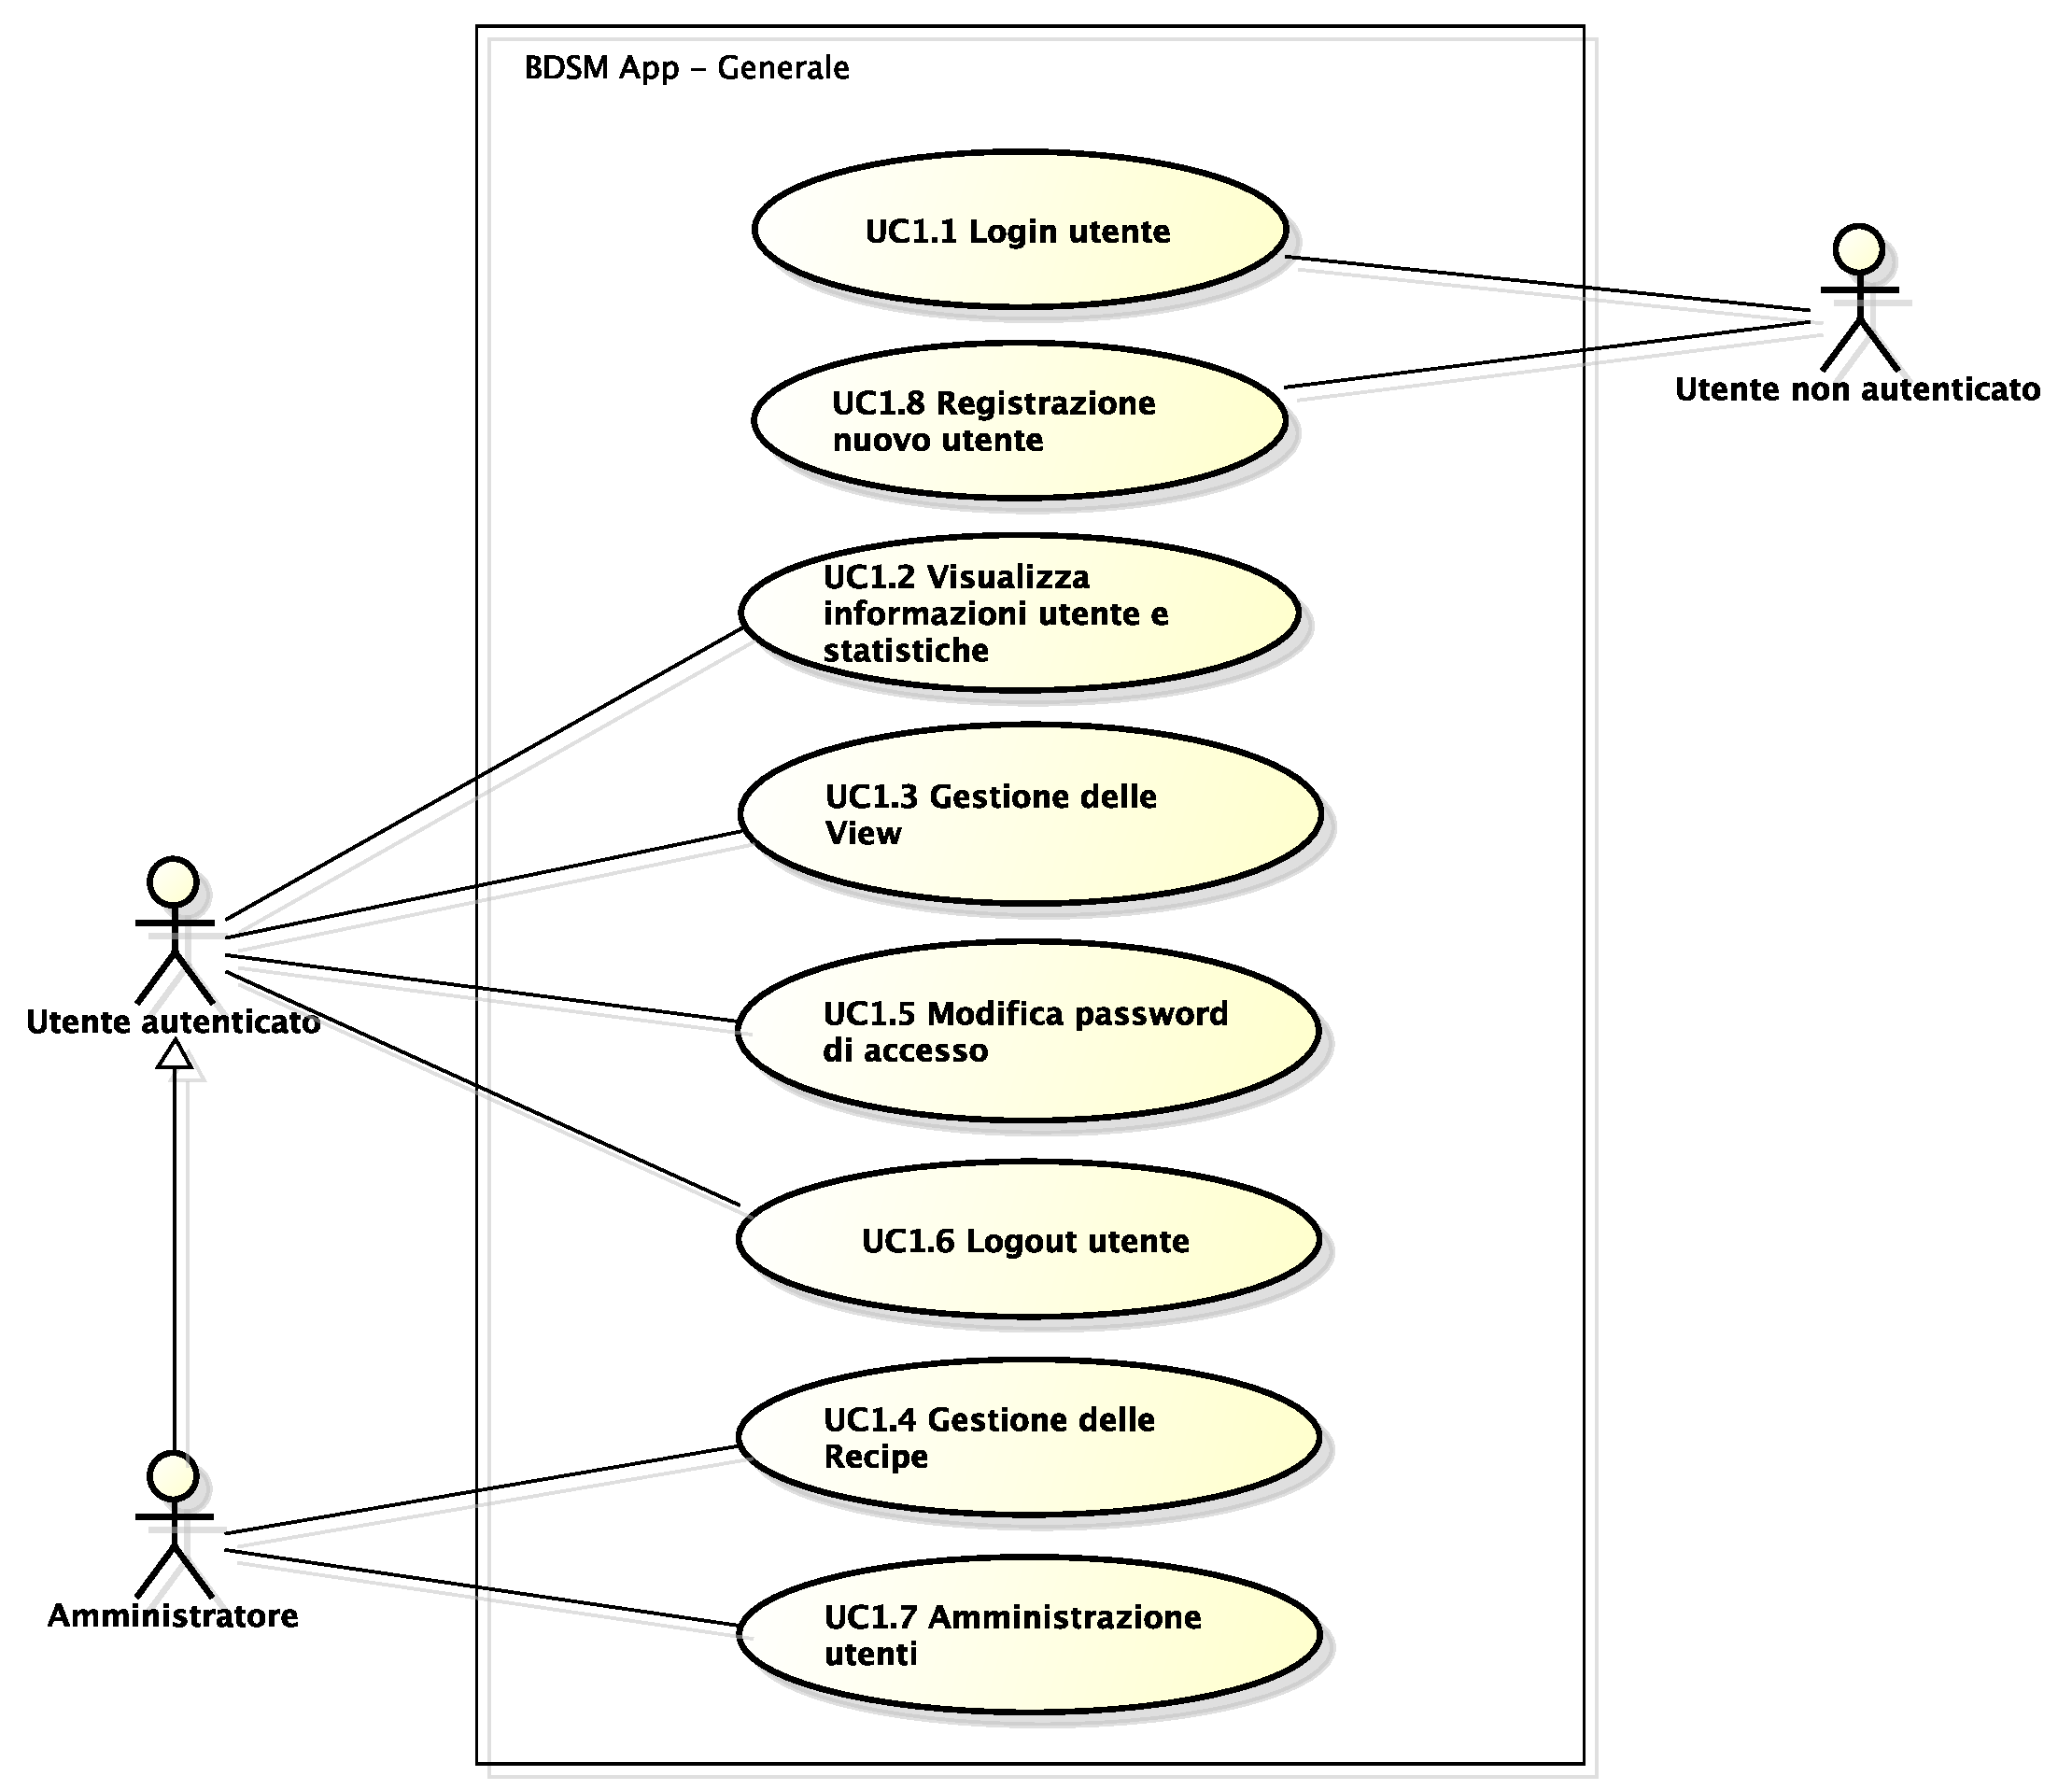
\includegraphics[scale=0.45]{./images/UC1.pdf}}
    \caption{UC1 - Caso d'uso pubblico}
\end{figure}

\begin{itemize}
    \item \textbf{Attori:}
    \begin{itemize}
    	\item utente sconosciuto: utente non autenticato che accede al servizio;
    	\item utente autenticato: utente autenticato che ha accesso al servizio;
    	\item utente amministratore: utente autenticato che ha accesso al servizio e dispone dei permessi per visualizzare tutte le aree;
	\end{itemize}
    \item \textbf{Descrizione:} dopo l'accesso al servizio:
    \begin{itemize}
    	\item un utente sconosciuto può autenticarsi, o se è al primo accesso al servizio può registrarsi per ottenere delle credenziali valide;
    	\item un utente autenticato può vedere statistiche, modificare la propria password, visualizzare, creare e modificare le proprie View\gloss{};
  		\item un utente amministratore può fare tutte le operazioni di un utente autenticato, più ha la possibilità di eliminare un utente e tutte le sue View\gloss{} e modificarne i privilegi;
	\end{itemize}
    \item \textbf{Precondizione:} l'utente autenticato, l'utente non autenticato o l'amministratore hanno caricato la prima pagina del servizio;
    Viene visualizzato un messaggio di errore nel caso le informazioni di accesso inserite siano errate;
    \item \textbf{Postcondizione:} il servizio ha erogato correttamente le funzionalità richieste dall'utente;
    \item \textbf{Flusso principale degli eventi:}
    	\begin{enumerate}
    		\item Login utente (UC1.1);
    		\item Visualizza informazione utente e statistiche (UC1.2);
    		\item Gestione delle View\gloss{} (UC1.3);
    		\item Gestione delle Recipe\gloss{} (UC1.4);
    		\item Modifica password di accesso (UC1.5);
    		\item Logout utente (UC1.6);
    		\item Amministrazione utenti (UC1.7);
    		\item Registrazione nuovo utente (UC1.8);
    	\end{enumerate}
\end{itemize}

\pagebreak

\subsection{UC1.1: Login utente}

\begin{figure}[htbp]
    \centering
    \centerline{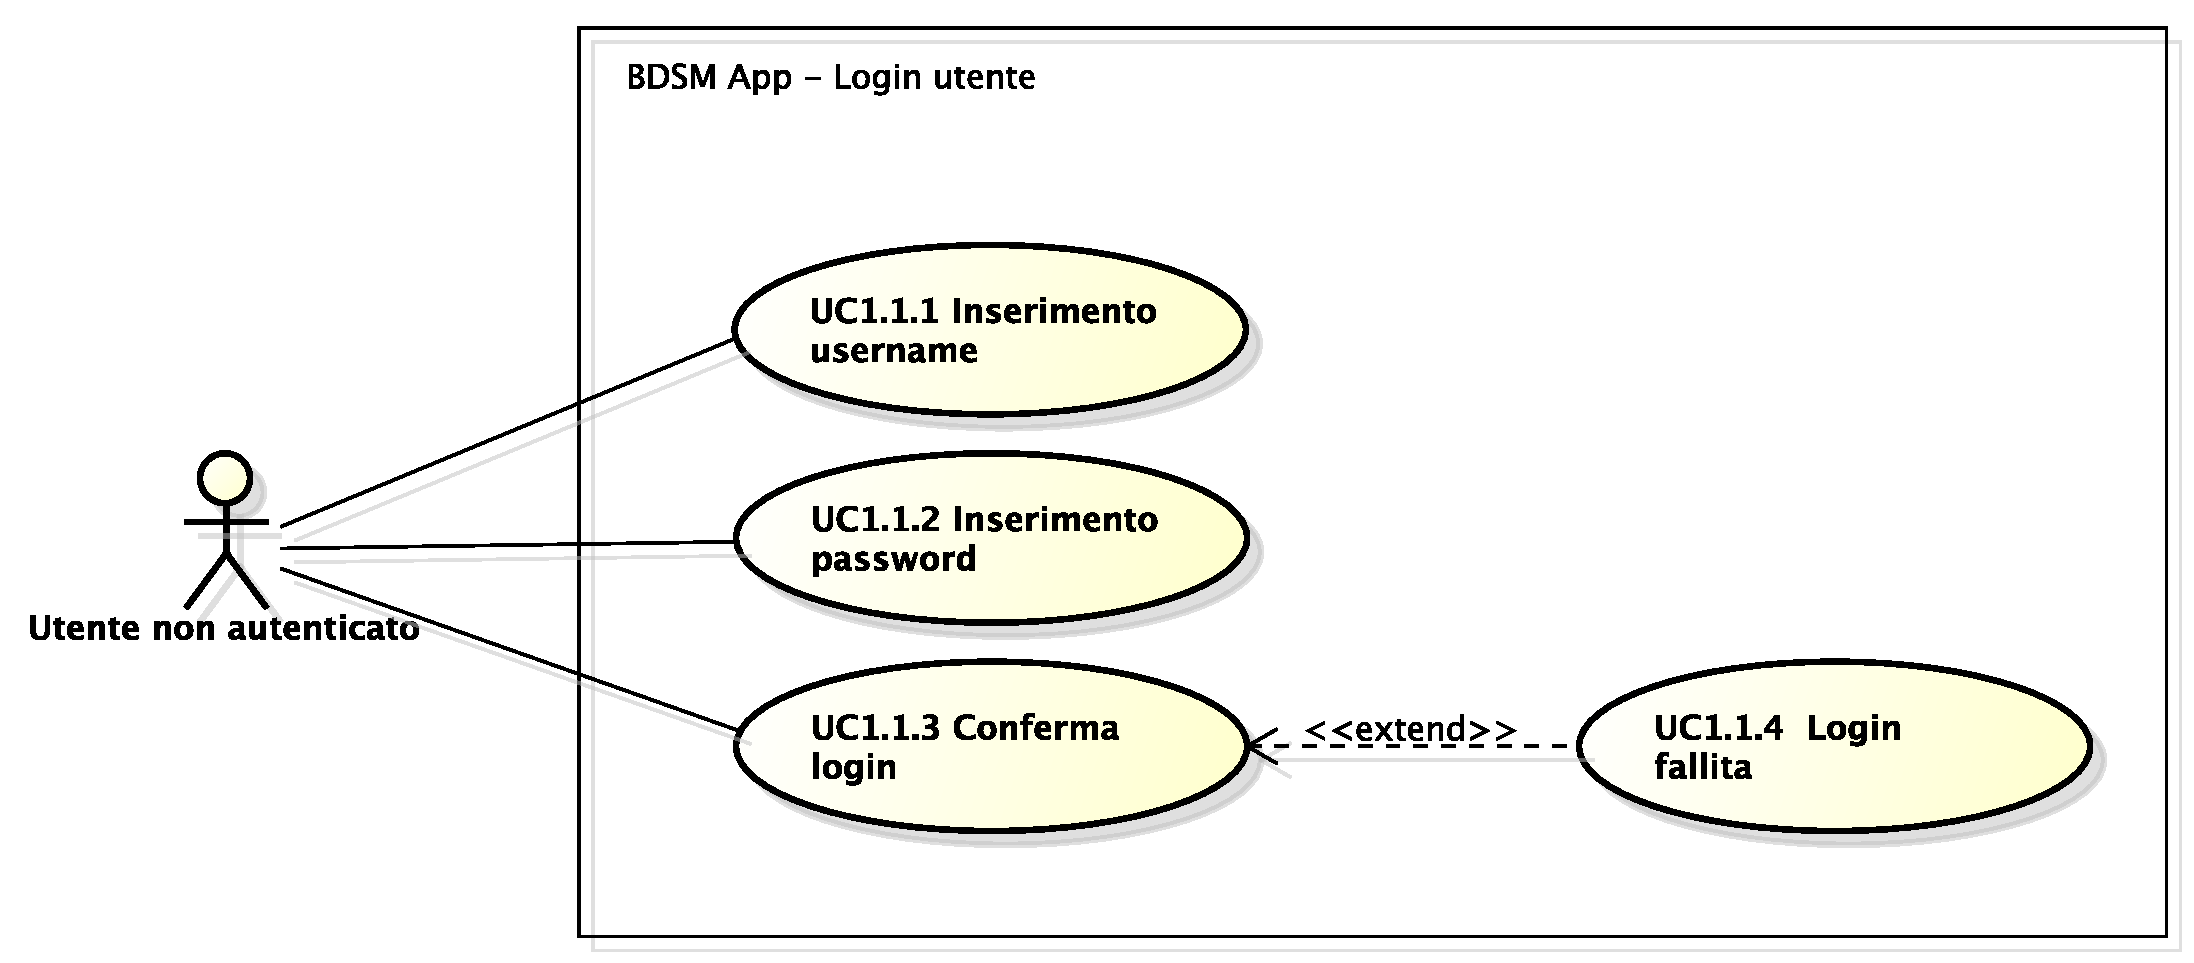
\includegraphics[scale=0.45]{./images/UC1_1.pdf}}
    \caption{UC1.1 - Login utente}
\end{figure}

\begin{itemize}
    \item \textbf{Attori:}
    \begin{itemize}
        \item utente sconosciuto: utente non autenticato che accede al servizio;
    \end{itemize}
    \item \textbf{Descrizione:} l'utente può autenticarsi per poter accedere ai servizi offerti dalla piattaforma utilizzando la schermata di login;
    \item \textbf{Precondizione:} l'utente che accede alla pagina di accesso è sconosciuto al sistema;
    \item \textbf{Postcondizione:} l'utente è riconosciuto dal sistema;
    \item \textbf{Flusso principale degli eventi:}
    \begin{enumerate}
        \item Inserimento username (UC1.1.1);
        \item Inserimento password (UC1.1.2);
        \item Conferma login (UC1.1.3);
    \end{enumerate}
    \item \textbf{Estensioni:} Login fallita (UC1.1.4).
\end{itemize}


\subsubsection{UC1.1.1: Inserimento username}

\begin{itemize}
    \item \textbf{Attori:}
    \begin{itemize}
        \item utente sconosciuto: utente non autenticato che accede al servizio;
    \end{itemize}
    \item \textbf{Descrizione:} l'utente non autenticato inserisce l'username;
    \item \textbf{Precondizione:} il sistema fornisce una schermata in cui è possibile inserire l’username;
    \item \textbf{Postcondizione:} il sistema ha l'informazione relativa all'username.
\end{itemize}

\subsubsection{UC1.1.2: Inserimento password}

\begin{itemize}
    \item \textbf{Attori:}
    \begin{itemize}
        \item utente sconosciuto: utente non autenticato che accede al servizio;
    \end{itemize}
    \item \textbf{Descrizione:} l'utente non autenticato inserisce la propria password personale;
    \item \textbf{Precondizione:} il sistema fornisce una schermata in cui è possibile inserire la password;
    \item \textbf{Postcondizione:} il sistema ha l'informazione relativa alla password inserita dall'utente.
\end{itemize}

\subsubsection{UC1.1.3: Conferma login}

\begin{itemize}
    \item \textbf{Attori:}
    \begin{itemize}
        \item utente sconosciuto: utente non autenticato che accede al servizio;
    \end{itemize}
    \item \textbf{Descrizione:} viene richiesto all'utente di confermare i dati inseriti con la pressione di un pulsante di conferma;
    \item \textbf{Precondizione:} il sistema fornisce un pulsante per confermare il login;
    \item \textbf{Postcondizione:} l'utente ha eseguito il login.
\end{itemize}

\subsubsection{UC1.1.4: Login fallita}

\begin{itemize}
    \item \textbf{Attori:}
    \begin{itemize}
        \item utente sconosciuto: utente non autenticato che accede al servizio;
    \end{itemize}
    \item \textbf{Descrizione:} viene mostrato all'utente un messaggio di errore che riporta l'incorrettezza dei dati inseriti. Viene visualizzato un pulsante per tornare alla schermata di login;
    \item \textbf{Precondizione:} il sistema ha ricevuto una richiesta di accesso con dati errati;
    \item \textbf{Postcondizione:} l'utente ha preso atto del messaggio di errore.
\end{itemize}

\pagebreak

\subsection{UC1.2: Visione informazioni utente e statistiche}

\begin{figure}[htbp]
    \centering
    \centerline{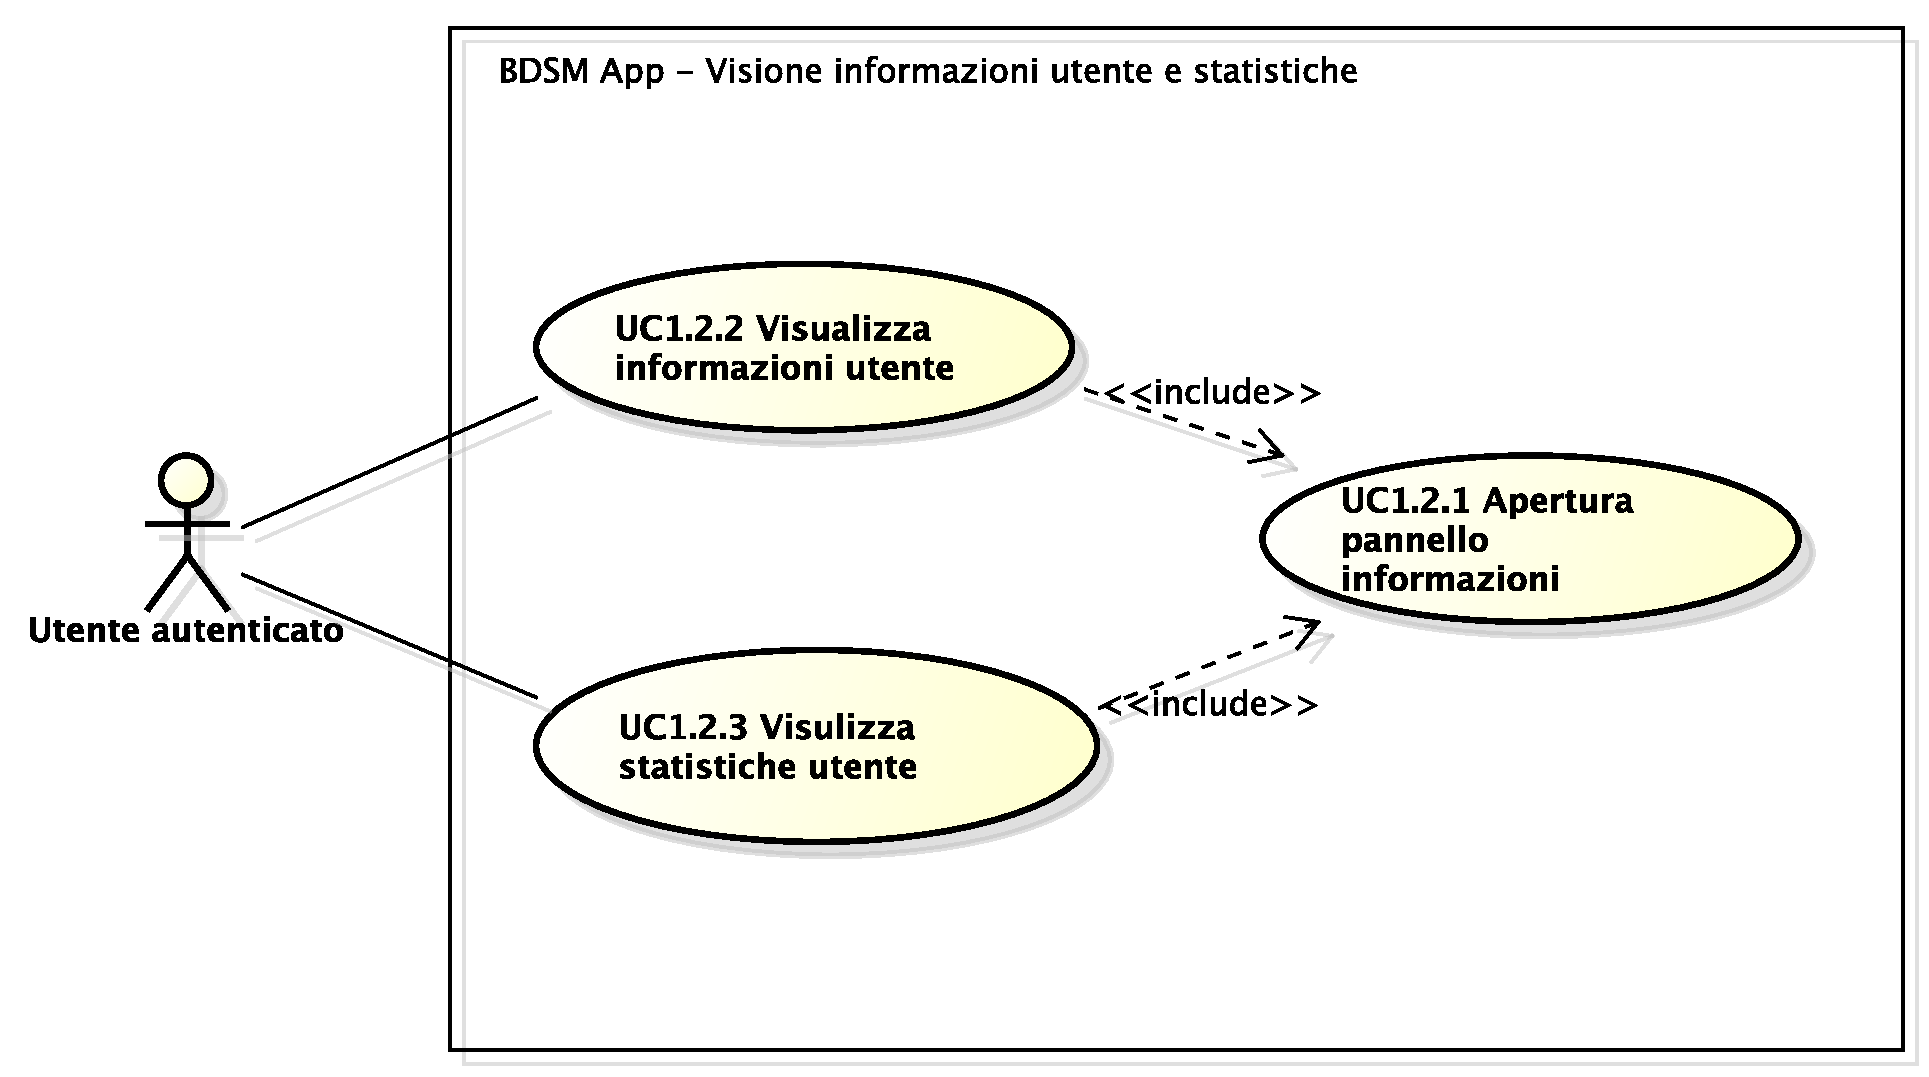
\includegraphics[scale=0.45]{./images/UC1_2.pdf}}
    \caption{UC1.2 - Visione informazioni utente e statistiche}
\end{figure}

\begin{itemize}
    \item \textbf{Attori:}
    \begin{itemize}
        \item utente autenticato: utente autenticato che ha accesso al servizio;
        \item utente amministratore: utente autenticato che ha accesso al servizio e dispone dei permessi per visualizzare tutte le aree;
    \end{itemize}
    \item \textbf{Descrizione:} gli utenti autenticati possono vedere una serie di informazioni relative alla 	loro attività, come la data dell'ultimo accesso effettuato e il numero di ricette e viste attive;
    \item \textbf{Precondizione:} l'utente deve essere autenticato;
    \item \textbf{Postcondizione:} le informazioni richieste dall'utente sono state fornite;
    \item \textbf{Flusso principale degli eventi:}
    \begin{enumerate}
        \item Apertura pannello informazioni (UC1.2.1);
        \item Visualizza informazioni utente (UC1.2.2);
        \item Visualizza statistiche utente (UC1.2.3).
    \end{enumerate}
\end{itemize}

\subsubsection{UC1.2.1: Apertura pannello informazioni}

\begin{itemize}
    \item \textbf{Attori:}
    \begin{itemize}
        \item utente autenticato: utente autenticato che ha accesso al servizio;
        \item utente amministratore: utente autenticato che ha accesso al servizio e dispone dei permessi per visualizzare tutte le aree;
    \end{itemize}
    \item \textbf{Descrizione:} dalla home screen dell'utente è possibile accedere al pannello informazioni e statistiche attinenti all'utente attualmente connesso;
    \item \textbf{Precondizione:} l'utente ha eseguito l'accesso al sistema;
    \item \textbf{Postcondizione:} l'utente ha visualizzato il contenuto del pannello.
\end{itemize}

\subsubsection{UC1.2.2: Visualizza informazioni utente}

\begin{itemize}
    \item \textbf{Attori:}
    \begin{itemize}
        \item utente autenticato: utente autenticato che ha accesso al servizio;
        \item utente amministratore: utente autenticato che ha accesso al servizio e dispone dei permessi per visualizzare tutte le aree;
    \end{itemize}
    \item \textbf{Descrizione:} selezionando il pulsante informazioni viene mostrata all'utente una pagina con il riepilogo dei sui dati, quali:
    \begin{itemize}
        \item il nome utente;
        \item l'indirizzo email associato;
        \item la data dell'ultimo accesso effettuato;
    \end{itemize}
    \item \textbf{Precondizione:} l'utente ha selezionato il pulsante di visualizzazione informazioni;
    \item \textbf{Postcondizione:} l'utente ha ottenuto le informazioni richieste.
\end{itemize}

\subsubsection{UC1.2.3: Visualizza statistiche utente}

\begin{itemize}
    \item \textbf{Attori:}
    \begin{itemize}
        \item utente autenticato: utente autenticato che ha accesso al servizio;
        \item utente amministratore: utente autenticato che ha accesso al servizio e dispone dei permessi per visualizzare tutte le aree;
    \end{itemize}
    \item \textbf{Descrizione:} selezionando il pulsante statistiche viene mostrata all'utente una pagina con il riepilogo delle sue statistiche, quali:
    \begin{itemize}
        \item numero di View\gloss{} attive;
        \item numero di Recipe\gloss{} disponibili;
        \item numero di accessi negli ultimi 30 giorni;
    \end{itemize}
    \item \textbf{Precondizione:} l'utente ha selezionato il pulsante di visualizzazione statistiche;
    \item \textbf{Postcondizione:} l'utente ha ottenuto le informazioni richieste.
\end{itemize}

\pagebreak
\subsection{UC1.3: Gestione delle View}

\begin{figure}[!htbp]
    \centering
    \centerline{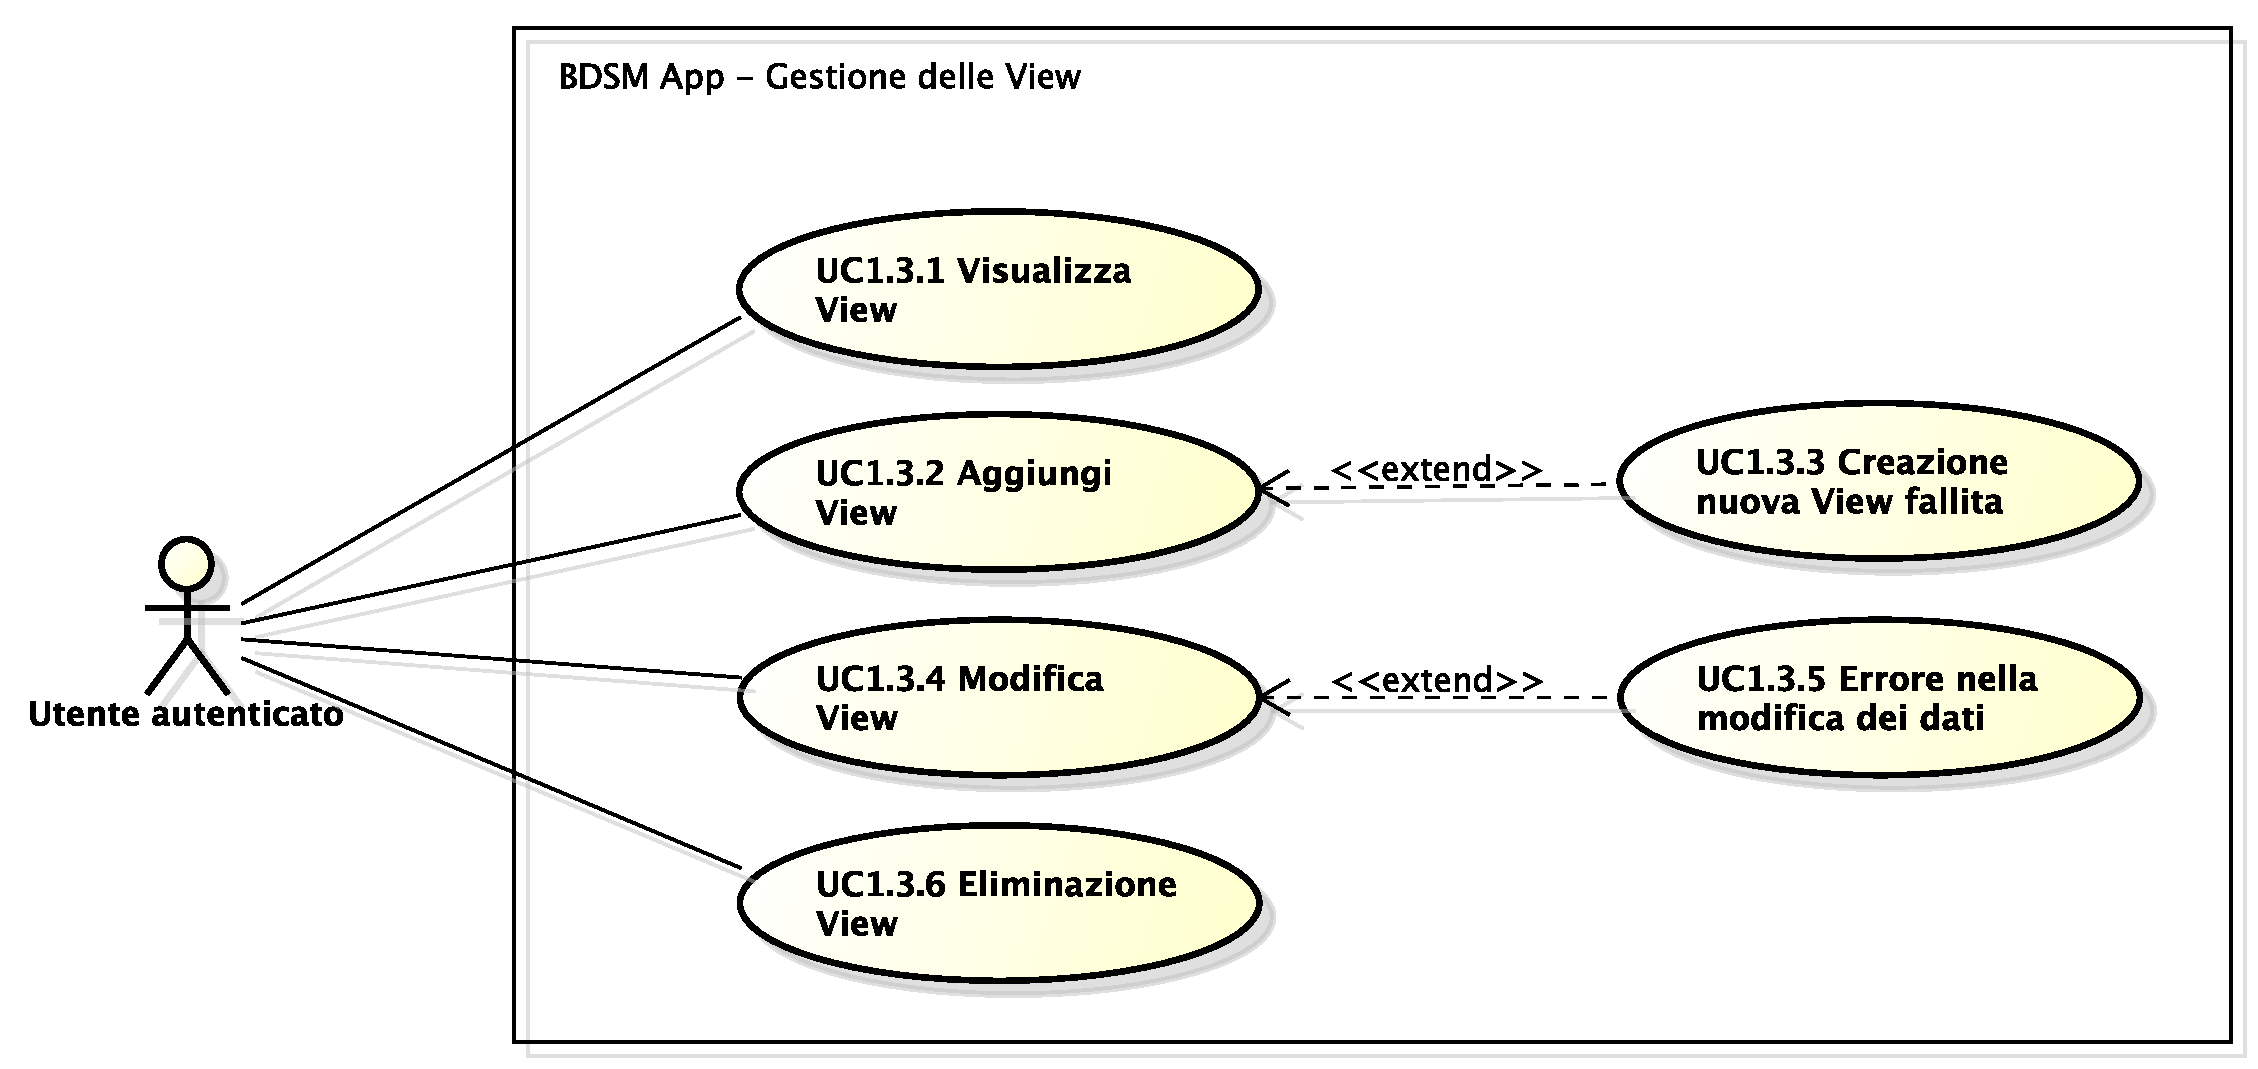
\includegraphics[scale=0.45]{./images/UC1_3.pdf}}
    \caption{UC1.3 - Gestione delle View}
\end{figure}

\begin{itemize}
    \item \textbf{Attori:}
    \begin{itemize}
    	\item utente autenticato: utente autenticato che ha accesso al servizio;
    	\item utente amministratore: utente autenticato che ha accesso al servizio e dispone dei permessi per visualizzare tutte le aree;
	\end{itemize}
	 \item \textbf{Descrizione:} gli utenti possono vedere in questa pagina le View\gloss{} e i dati ad esse associate. Per ciascuna View è disponibile un pannello per modificarne i parametri, in oltre si può creare una nuova View o eliminarne una esistente.
    \item \textbf{Precondizione:} l'utente deve aver fatto l'accesso nell'apposita pagina;
    \item \textbf{Postcondizione:} le informazioni richieste dall'utente sono state fornite, le impostazioni modificate sono state salvate nel sistema e le informazioni aggiunte sono state salvate;
    \item \textbf{Flusso principale degli eventi:}
    	\begin{enumerate}
    		\item Visualizza View\gloss{} (UC1.3.1);
    		\item Aggiungi View\gloss{} (UC1.3.2);
    		\item Modifica View\gloss{} (UC1.3.4);
    		\item Eliminazione View\gloss{} (UC1.3.6);
    	\end{enumerate}
    \item \textbf{Estensioni:}
    \begin{itemize}
    	\item Creazione nuova View\gloss{} fallita (UC1.3.3);
    	\item Errore nella modifica dei dati (UC1.3.5).
	\end{itemize}
\end{itemize}

\subsubsection{UC1.3.1: Visualizza View}

\begin{itemize}
    \item \textbf{Attori:}
    \begin{itemize}
    	\item utente autenticato: utente autenticato che ha accesso al servizio;
    	\item utente amministratore: utente autenticato che ha accesso al servizio e dispone dei permessi per visualizzare tutte le aree;
	\end{itemize}
    \item \textbf{Descrizione:} questa è la home screen dell'utente attualmente connesso qui, potrà visualizzare tutte le sue View\gloss{} e accedere ai menu di configurazione;
    \item \textbf{Precondizione:} l'utente ha effettuato il login e ha selezionato il pulsante per accedere a questa pagina;
    \item \textbf{Postcondizione:} l'utente viene reindirizzato alla home screen e visualizza le informazioni richieste;
	\item \textbf{Flusso principale degli eventi:}
		\begin{enumerate}
			\item Apertura elenco View\gloss{} (UC1.3.1.1).
		\end{enumerate}
\end{itemize}
\subsubsection{UC1.3.1.1: Apertura elenco View}

\begin{itemize}
    \item \textbf{Attori:}
    \begin{itemize}
    	\item utente autenticato: utente autenticato che ha accesso al servizio;
    	\item utente amministratore: utente autenticato che ha accesso al servizio e dispone dei permessi per visualizzare tutte le aree;
	\end{itemize}
    \item \textbf{Descrizione:} premendo sull'apposito pulsante è possibile far comparire a video l'elenco di tutte le View\gloss{} utente;
    \item \textbf{Precondizione:} l'utente si trova nella home screen;
    \item \textbf{Postcondizione:} l'utente ha ottenuto l'elenco di tutte le sue View\gloss{}.
\end{itemize}

\subsubsection{UC1.3.2: Aggiungi View}

\begin{itemize}
    \item \textbf{Attori:}
    \begin{itemize}
    	\item utente autenticato: utente autenticato che ha accesso al servizio;
    	\item utente amministratore: utente autenticato che ha accesso al servizio e dispone dei permessi per visualizzare tutte le aree;
	\end{itemize}
    \item \textbf{Descrizione:} dalla home screen l'utente può aggiungere una nuova View\gloss{} premendo sull'apposito pulsante e compilando i dati richiesti;
    \item \textbf{Precondizione:} l'utente si è autenticato e si trova nella home screen;
    \item \textbf{Postcondizione:} l'utente ha creato una nuovo View\gloss{};
	\item \textbf{Flusso principale degli eventi:}
    \begin{enumerate}
        \item Apertura pannello (UC1.3.2.1);
        \item Inserimento parametri (UC1.3.2.2);
        \item Conferma creazione View\gloss{} (UC1.3.2.3).
    \end{enumerate}
\end{itemize}

\subsubsection{UC1.3.2.1: Apertura pannello}

\begin{itemize}
    \item \textbf{Attori:}
    \begin{itemize}
    	\item utente autenticato: utente autenticato che ha accesso al servizio;
    	\item utente amministratore: utente autenticato che ha accesso al servizio e dispone dei permessi per visualizzare tutte le aree;
	\end{itemize}
    \item \textbf{Descrizione:} l'utente ha a disposizione un pulsante per aprire il pannello in cui inserire e selezionare i dati per la creazione di una nuova View\gloss{};
    \item \textbf{Precondizione:} l'utente si trova nella home screen;
    \item \textbf{Postcondizione:} l'utente ha aperto il pannello di creazione di una nuova View\gloss{}.
\end{itemize}

\subsubsection{UC1.3.2.2: Inserimento parametri}

\begin{itemize}
    \item \textbf{Attori:}
    \begin{itemize}
    	\item utente autenticato: utente autenticato che ha accesso al servizio;
    	\item utente amministratore: utente autenticato che ha accesso al servizio e dispone dei permessi per visualizzare tutte le aree;
	\end{itemize}
    \item \textbf{Descrizione:} l'utente può inserire il nome, i parametri obbligatori e facoltativi relativi ad una nuova View\gloss{};
    \item \textbf{Precondizione:} l'utente ha aperto il pannello di inserimento di una nuova View\gloss{};
    \item \textbf{Postcondizione:} l'utente ha inserito le informazioni richieste.
\end{itemize}

\subsubsection{UC1.3.2.3: Conferma creazione View}

\begin{itemize}
    \item \textbf{Attori:}
    \begin{itemize}
    	\item utente autenticato: utente autenticato che ha accesso al servizio;
    	\item utente amministratore: utente autenticato che ha accesso al servizio e dispone dei permessi per visualizzare tutte le aree;
	\end{itemize}
    \item \textbf{Descrizione:} l'utente è tenuto a confermare i parametri inseriti nel pannello di creazione di una nuova View\gloss{} prima di poter utilizzare il grafico associato.
    \item \textbf{Precondizione:} l'utente ha inserito almeno i parametri obbligatori;
    \item \textbf{Postcondizione:} l'utente ha confermato i parametri inseriti e la View\gloss{} è stata salvata nel sistema;
\end{itemize}

\subsubsection{UC1.3.3: Creazione nuova View fallita}

\begin{itemize}
   	\item \textbf{Attori:}
    \begin{itemize}
    	\item utente autenticato: utente autenticato che ha accesso al servizio;
    	\item utente amministratore: utente autenticato che ha accesso al servizio e dispone dei permessi per visualizzare tutte le aree;
	\end{itemize}
    \item \textbf{Descrizione:} nel caso i dati inseriti non rispettino i vincoli del sistema oppure se si verifica un errore lato server, viene visualizzata questa pagina di errore con una breve descrizione dell'anomalia rilevata;
    \item \textbf{Precondizione:} l'utente ha inserito dei dati che non rispettano i vincoli del sistema. Il server ha sollevato un'eccezione durante il salvataggio dei dati;
    \item \textbf{Postcondizione:} nessuna modifica richiesta è stata salvata nel sistema.
\end{itemize}

\subsubsection{UC1.3.4: Modifica View}

\begin{itemize}
   	\item \textbf{Attori:}
    \begin{itemize}
    	\item utente autenticato: utente autenticato che ha accesso al servizio;
    	\item utente amministratore: utente autenticato che ha accesso al servizio e dispone dei permessi per visualizzare tutte le aree;
	\end{itemize}
    \item \textbf{Descrizione:} l'utente può modificare i parametri di una View\gloss{};
    \item \textbf{Precondizione:} la View\gloss{} è stata creata ed è disponibile nell'elenco delle View dell'utente;
    \item \textbf{Postcondizione:} i parametri della View\gloss{} selezionata sono stati modificati;
	\item \textbf{Flusso principale degli eventi:}
    \begin{enumerate}
        \item Selezione di una View\gloss{} (UC1.3.4.1);
        \item Selezione tasto modifica (UC1.3.4.2);
        \item Inserimento nuovi parametri (UC1.3.4.3);
        \item Conferma nuovi parametri (UC1.3.4.4).
    \end{enumerate}
\end{itemize}

\subsubsection{UC1.3.4.1: Selezione di una View}

\begin{itemize}
    \item \textbf{Attori:}
    \begin{itemize}
    	\item utente autenticato: utente autenticato che ha accesso al servizio;
    	\item utente amministratore: utente autenticato che ha accesso al servizio e dispone dei permessi per visualizzare tutte le aree;
	\end{itemize}
    \item \textbf{Descrizione:} l'utente deve selezionare la View\gloss{} desiderata dall'elenco delle View per poterla visualizzare e modificare;
    \item \textbf{Precondizione:} l'utente si trova nel suo elenco delle View\gloss{};
    \item \textbf{Postcondizione:} l'utente ha selezionato e visualizzato la View\gloss{} desiderata.
\end{itemize}

\subsubsection{UC1.3.4.2: Selezione tasto modifica}

\begin{itemize}
   	\item \textbf{Attori:}
    \begin{itemize}
    	\item utente autenticato: utente autenticato che ha accesso al servizio;
    	\item utente amministratore: utente autenticato che ha accesso al servizio e dispone dei permessi per visualizzare tutte le aree;
	\end{itemize}
    \item \textbf{Descrizione:} l'utente può selezionare il pulsante modifica dal pannello della View\gloss{} attualmente visualizzata per modificarne i parametri;
    \item \textbf{Precondizione:} l'utente ha visualizzato correttamente una View\gloss{};
    \item \textbf{Postcondizione:} l'utente ha aperto il pannello modifica View\gloss{}.
\end{itemize}

\subsubsection{UC1.3.4.3: Inserimento nuovi parametri}

\begin{itemize}
    \item \textbf{Attori:}
    \begin{itemize}
    	\item utente autenticato: utente autenticato che ha accesso al servizio;
    	\item utente amministratore: utente autenticato che ha accesso al servizio e dispone dei permessi per visualizzare tutte le aree;
	\end{itemize}
    \item \textbf{Descrizione:} l'utente può inserire i nuovi parametri della View\gloss{} aggiungendoli a quelli esistenti oppure sovrascrivendoli;
    \item \textbf{Precondizione:} l'utente ha visualizzato il pannello modifica View\gloss{};
    \item \textbf{Postcondizione:} l'utente ha inserito i nuovi parametri.
\end{itemize}

\subsubsection{UC1.3.4.4: Conferma nuovi parametri}

\begin{itemize}
    \item \textbf{Attori:}
    \begin{itemize}
    	\item utente autenticato: utente autenticato che ha accesso al servizio;
    	\item utente amministratore: utente autenticato che ha accesso al servizio e dispone dei permessi per visualizzare tutte le aree;
	\end{itemize}
    \item \textbf{Descrizione:} l'utente deve confermare i parametri inseriti prima che questi siano salvati;
    \item \textbf{Precondizione:} l'utente ha inserito i parametri desiderati;
    \item \textbf{Postcondizione:} i nuovi parametri sono stati memorizzati nel sistema e attivi.
\end{itemize}

\subsubsection{UC1.3.5: Errore nella modifica dei dati}

\begin{itemize}
    \item \textbf{Attori:}
    \begin{itemize}
    	\item utente autenticato: utente autenticato che ha accesso al servizio;
    	\item utente amministratore: utente autenticato che ha accesso al servizio e dispone dei permessi per visualizzare tutte le aree;
	\end{itemize}
    \item \textbf{Descrizione:} l'utente visualizza una schermata di errore con i parametri che ha inserito non conformi ai vincoli di sistema;
    \item \textbf{Precondizione:} l'utente ha inserito dei parametri non validi;
    \item \textbf{Postcondizione:} l'utente ha visualizzato il messaggio di errore e ha preso atto dei parametri non conformi ai vincoli di sistema.
\end{itemize}

\subsubsection{UC1.3.6: Eliminazione View}

\begin{itemize}
    \item \textbf{Attori:}
    \begin{itemize}
    	\item utente autenticato: utente autenticato che ha accesso al servizio;
    	\item utente amministratore: utente autenticato che ha accesso al servizio e dispone dei permessi per visualizzare tutte le aree;
	\end{itemize}
    \item \textbf{Descrizione:} l'utente può eliminare una View\gloss{} precedentemente creata;
    \item \textbf{Precondizione:} l'utente ha creato almeno una View\gloss{} ed è visibile nel suo elenco;
    \item \textbf{Postcondizione:} l'utente ha cancellato una View\gloss{} dal suo elenco;
    \item \textbf{Flusso principale degli eventi:}
    \begin{enumerate}
        \item Selezione View\gloss{} (UC1.3.6.1);
        \item Eliminazione View\gloss{} (UC1.3.6.2);
        \item Conferma eliminazione View\gloss{} (UC1.3.6.3).
    \end{enumerate}
\end{itemize}

\subsubsection{UC1.3.6.1: Selezione View}

\begin{itemize}
 	\item \textbf{Attori:}
    \begin{itemize}
    	\item utente autenticato: utente autenticato che ha accesso al servizio;
    	\item utente amministratore: utente autenticato che ha accesso al servizio e dispone dei permessi per visualizzare tutte le aree;
	\end{itemize}
    \item \textbf{Descrizione:} l'utente deve selezionare la View\gloss{} desiderata dal suo elenco per poterla visualizzare e modificare;
    \item \textbf{Precondizione:} l'utente si trova nel suo elenco delle View\gloss{};
    \item \textbf{Postcondizione:} l'utente ha selezionato e visualizzato la View\gloss{} desiderata.
\end{itemize}

\subsubsection{UC1.3.6.2: Eliminazione View}

\begin{itemize}
   	\item \textbf{Attori:}
    \begin{itemize}
    	\item utente autenticato: utente autenticato che ha accesso al servizio;
    	\item utente amministratore: utente autenticato che ha accesso al servizio e dispone dei permessi per visualizzare tutte le aree;
	\end{itemize}
    \item \textbf{Descrizione:} l'utente può selezionare il pulsante per eliminare la View\gloss{} visualizzata;
    \item \textbf{Precondizione:} l'utente ha visualizzato correttamente una View\gloss{};
    \item \textbf{Postcondizione:} l'utente ha selezionato il pulsante per eliminare la View\gloss{}.
\end{itemize}

\subsubsection{UC1.3.6.3: Conferma eliminazione View}

\begin{itemize}
   	\item \textbf{Attori:}
    \begin{itemize}
    	\item utente autenticato: utente autenticato che ha accesso al servizio;
    	\item utente amministratore: utente autenticato che ha accesso al servizio e dispone dei permessi per visualizzare tutte le aree;
	\end{itemize}
    \item \textbf{Descrizione:} l'utente deve confermare l'eliminazione della View\gloss{} selezionando il pulsante di conferma;
    \item \textbf{Precondizione:} l'utente ha selezionato il pulsante per eliminare una View\gloss{};
    \item \textbf{Postcondizione:} l'utente ha confermato l'eliminazione e la View\gloss{} è stata eliminata dal sistema.
\end{itemize}

\pagebreak


\subsection{UC1.4: Gestione delle Recipe}

\begin{figure}[!ht]
    \centering
    \centerline{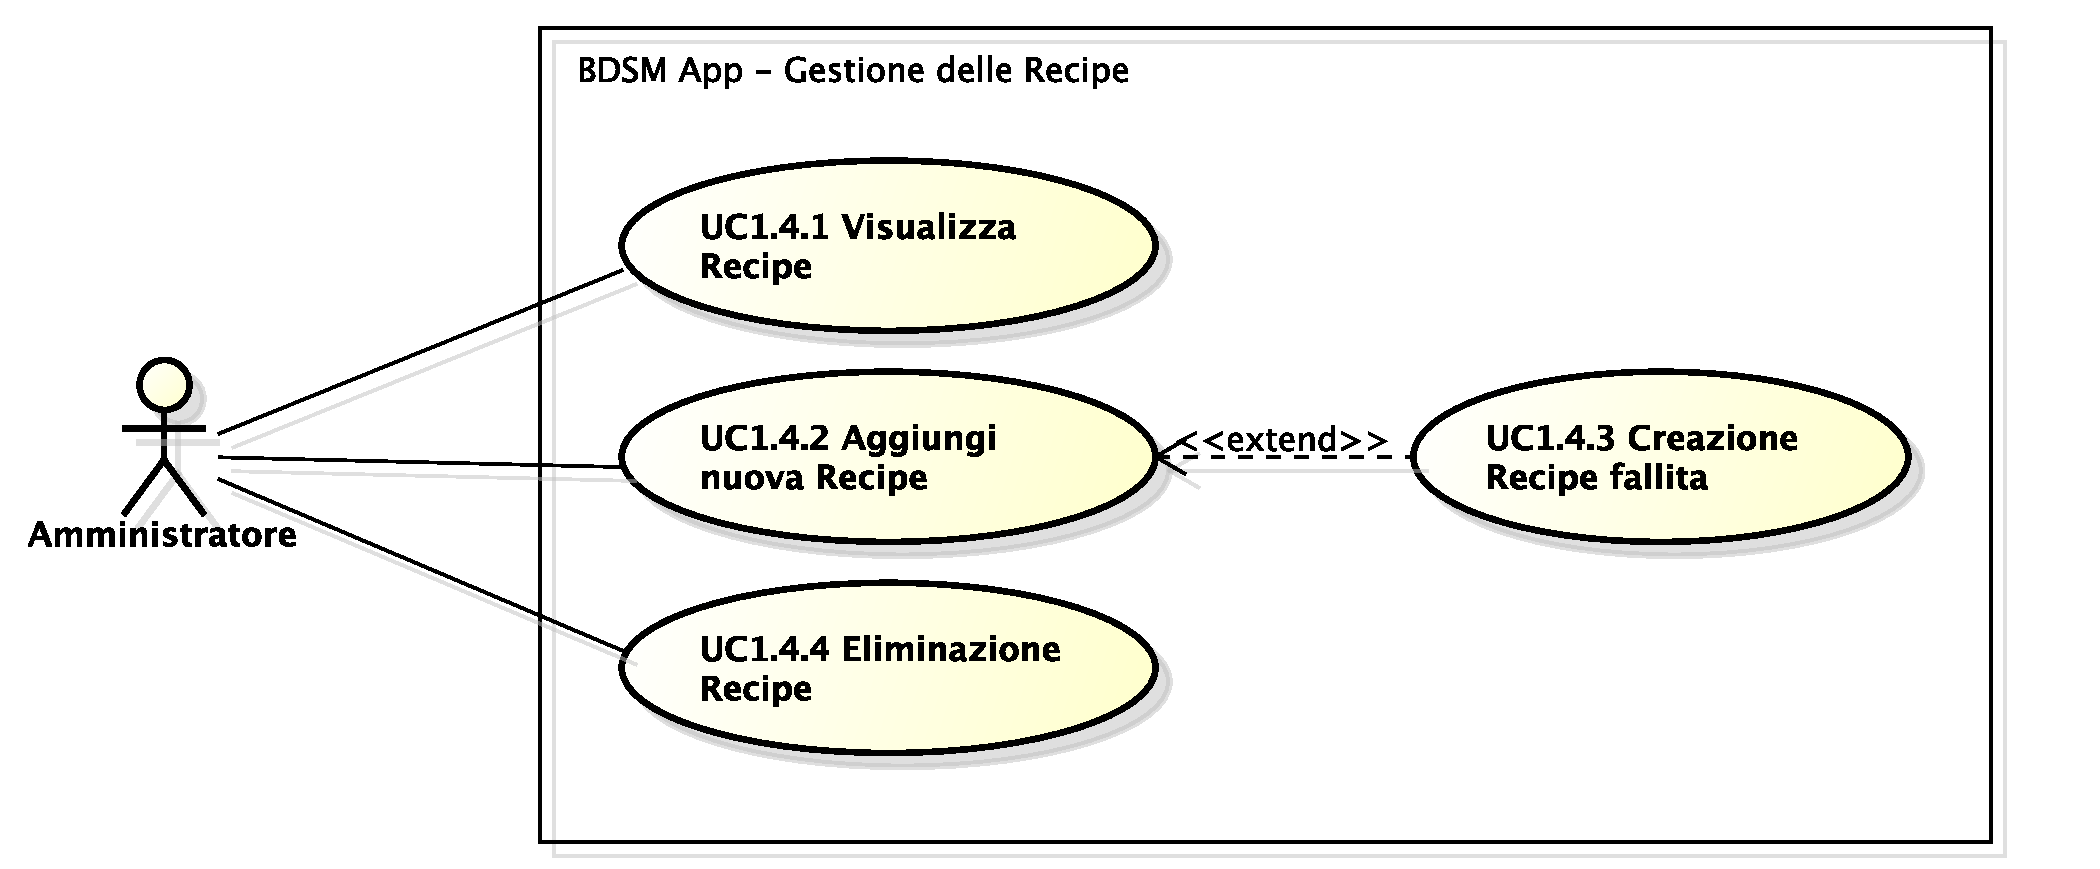
\includegraphics[scale=0.45]{./images/UC1_4.pdf}}
    \caption{UC1.4 - Gestione delle Recipe}
\end{figure}

\begin{itemize}
    \item \textbf{Attori:} utente amministratore: utente autenticato che ha accesso al servizio e dispone dei permessi per visualizzare tutte le aree;
    \item \textbf{Precondizione:} l'amministratore deve aver fatto il login nell'apposita pagina;
    \item \textbf{Descrizione:} gli amministratori possono vedere le Recipe\gloss{} e i dati ad esse associate. Possono inoltre crearle o eliminarle;
    \item \textbf{Postcondizione:} le informazioni richieste dall'amministratore sono state fornite, le Recipe\gloss{} eliminate, cancellate dal sistema e quelle aggiunte, salvate;
    \item \textbf{Flusso principale degli eventi:}
    \begin{enumerate}
        \item Visualizza Recipe\gloss{} (UC1.4.1);
        \item Aggiungi nuova Recipe\gloss{} (UC1.4.2);
        \item Elimina Recipe\gloss{} (UC1.4.4);
    \end{enumerate}
    \item \textbf{Estensioni:} Creazione Recipe\gloss{} fallita (UC1.4.3).
\end{itemize}

\subsubsection{UC1.4.1: Visualizza Recipe}

\begin{itemize}
    \item \textbf{Attori:} utente amministratore: utente autenticato che ha accesso al servizio e dispone dei permessi per visualizzare tutte le aree;
    \item \textbf{Descrizione:} l'amministratore può visualizzare l'elenco di tutte le Recipe\gloss{} salvate nel sistema selezionando l'apposito pulsante nella sua home screen;
    \item \textbf{Precondizione:} l'amministratore ha effettuato l'accesso al sistema e si trova nella sua home screen;
    \item \textbf{Postcondizione:} l'amministratore ha visualizzato correttamente l'elenco delle Recipe\gloss{} salvate nel sistema.
\end{itemize}

\subsubsection{UC1.4.2: Aggiungi nuova Recipe}
\begin{itemize}
    \item \textbf{Attori:} utente amministratore: utente autenticato che ha accesso al servizio e dispone dei permessi per visualizzare tutte le aree;
    \item \textbf{Descrizione:} l'amministratore può aggiungere una nuova Recipe\gloss{} al sistema;
    \item \textbf{Precondizione:} l'amministratore ha visualizzato l'elenco delle Recipe\gloss{} salvate nel sistema;
    \item \textbf{Postcondizione:} l'amministratore ha salvato una nuova Recipe\gloss{} nel sistema;
	\item \textbf{Flusso principale degli eventi:}
    \begin{enumerate}
        \item Apertura elenco Recipe\gloss{} (UC1.4.2.1);
        \item Apertura pannello inserimento nuova Recipe\gloss{} (UC1.4.2.2);
        \item Inserimento parametri (UC1.4.2.3);
        \item Conferma parametri inseriti (UC1.4.2.4).
    \end{enumerate}
\end{itemize}
\subsubsection{UC1.4.2.1: Apertura elenco Recipe}

\begin{itemize}
    \item \textbf{Attori:} utente amministratore: utente autenticato che ha accesso al servizio e dispone dei permessi per visualizzare tutte le aree;
    \item \textbf{Descrizione:} l'amministratore può visualizzare l'elenco delle Recipe\gloss{} salvate nel sistema premendo l'apposito pulsante nella sua Home Screen;
    \item \textbf{Precondizione:} l'amministratore ha effettuato l'accesso al sistema;
    \item \textbf{Postcondizione:} l'amministratore ha visualizzato correttamente l'elenco delle Recipe\gloss{}.
\end{itemize}

\subsubsection{UC1.4.2.2: Apertura pannello inserimento nuova Recipe}

\begin{itemize}
   	\item \textbf{Attori:} utente amministratore: utente autenticato che ha accesso al servizio e dispone dei permessi per visualizzare tutte le aree;
    \item \textbf{Descrizione:} l'amministratore può selezionare il pulsante di inserimento di una nuova Recipe\gloss{} dall'elenco delle Recipe;
    \item \textbf{Precondizione:} l'amministratore ha visualizzato l'elenco delle Recipe\gloss{};
    \item \textbf{Postcondizione:} l'amministratore ha visualizzato il pannello di inserimento nuova Recipe\gloss{}.
\end{itemize}

\subsubsection{UC1.4.2.3: Inserimento parametri}

\begin{itemize}
   	\item \textbf{Attori:} utente amministratore: utente autenticato che ha accesso al servizio e dispone dei permessi per visualizzare tutte le aree;
    \item \textbf{Descrizione:} l'amministratore può inserire il nome ed i parametri per la nuova Recipe\gloss{} nel pannello apposito;
    \item \textbf{Precondizione:} l'amministratore ha selezionato il pulsante per l'inserimento di una nuova Recipe\gloss{};
    \item \textbf{Postcondizione:} l'amministratore ha inserito tutti i parametri richiesti dal sistema.
\end{itemize}

\subsubsection{UC1.4.2.4: Conferma parametri inseriti}

\begin{itemize}
  	\item \textbf{Attori:} utente amministratore: utente autenticato che ha accesso al servizio e dispone dei permessi per visualizzare tutte le aree;
    \item \textbf{Descrizione:} l'amministratore deve confermare i parametri inseriti prima che questi siano attivi nel sistema;
    \item \textbf{Precondizione:} l'amministratore ha inserito almeno i parametri obbligatori;
    \item \textbf{Postcondizione:} l'amministratore ha confermato i parametri inseriti.
\end{itemize}

\subsubsection{UC1.4.3: Creazione Recipe fallita}

\begin{itemize}
  	\item \textbf{Attori:} utente amministratore: utente autenticato che ha accesso al servizio e dispone dei permessi per visualizzare tutte le aree;
    \item \textbf{Descrizione:} l'amministratore durante l'inserimento di una nuova Recipe\gloss{} ha inserito dei parametri che non rispettano i vincoli di sistema;
    \item \textbf{Precondizione:} l'amministratore ha selezionato il pulsante di conferma per la creazione di una nuova Recipe\gloss{};
    \item \textbf{Postcondizione:} l'amministratore ha visualizzato un messaggio di errore contenente l'elenco dei parametri inseriti non corretti o l'eccezione sollevata dal sistema durante il salvataggio della nuova Recipe\gloss{}.
\end{itemize}

\subsubsection{UC1.4.4: Eliminazione Recipe}

\begin{itemize}
  	\item \textbf{Attori:} utente amministratore: utente autenticato che ha accesso al servizio e dispone dei permessi per visualizzare tutte le aree;
    \item \textbf{Descrizione}: l'amministratore può eliminare una Recipe\gloss{} e tutti i dati ad essa associati.
    Si possono eliminare solo le Recipe\gloss{} non più utilizzate in una o più View\gloss{};
    \item \textbf{Precondizione:} l'amministratore deve aver visualizzato la schermata di gestione delle Recipe\gloss{};
    \item \textbf{Postcondizione:} le informazioni richieste dall'utente sono state fornite e la Recipe\gloss{} desiderata, con tutti i dati ad essa associati sono stati eliminati dal sistema;
    \item \textbf{Flusso principale degli eventi:}
    \begin{enumerate}
        \item Apertura elenco Recipe\gloss{} (UC1.4.4.1);
        \item Eliminazione Recipe\gloss{} (UC1.4.4.2);
        \item Conferma eliminazione Recipe\gloss{} (UC1.4.4.3).
    \end{enumerate}
\end{itemize}

\subsubsection{UC1.4.4.1: Apertura elenco Recipe}

\begin{itemize}
  	\item \textbf{Attori:} utente amministratore: utente autenticato che ha accesso al servizio e dispone dei permessi per visualizzare tutte le aree;
    \item \textbf{Descrizione:} l'amministratore può visualizzare l'elenco delle Recipe\gloss{} salvate nel sistema premendo l'apposito pulsante nella sua home screen;
    \item \textbf{Precondizione:} l'amministratore ha effettuato l'accesso al sistema;
    \item \textbf{Postcondizione:} l'amministratore ha visualizzato correttamente l'elenco delle Recipe\gloss{}.
\end{itemize}

\subsubsection{UC1.4.4.2: Eliminazione Recipe}

\begin{itemize}
  	\item \textbf{Attori:} utente amministratore: utente autenticato che ha accesso al servizio e dispone dei permessi per visualizzare tutte le aree;
    \item \textbf{Descrizione:} l'amministratore può selezionare il pulsante di eliminazione di una Recipe\gloss{} nell'elenco delle Recipe;
    \item \textbf{Precondizione:} l'amministratore ha visualizzato l'elenco delle Recipe\gloss{};
    \item \textbf{Postcondizione:} l'amministratore ha selezionato il pulsante di eliminazione di una Recipe\gloss{}.
\end{itemize}
\subsubsection{UC1.4.4.3: Conferma eliminazione Recipe}

\begin{itemize}
  	\item \textbf{Attori:} utente amministratore: utente autenticato che ha accesso al servizio e dispone dei permessi per visualizzare tutte le aree;
    \item \textbf{Descrizione:} l'amministratore deve confermare la volontà di eliminare la Recipe\gloss{} selezionando il pulsante di conferma eliminazione;
    \item \textbf{Precondizione:} l'amministratore ha selezionato il pulsante elimina su una Recipe\gloss{};
    \item \textbf{Postcondizione:} l'amministratore ha confermato l'eliminazione della Recipe\gloss{} e questa è stata cancellata dal sistema con a tutti i dati associati.
\end{itemize}

\pagebreak


\subsection{UC1.5: Modifica password di accesso}

\begin{figure}[!htbp]
    \centering
    \centerline{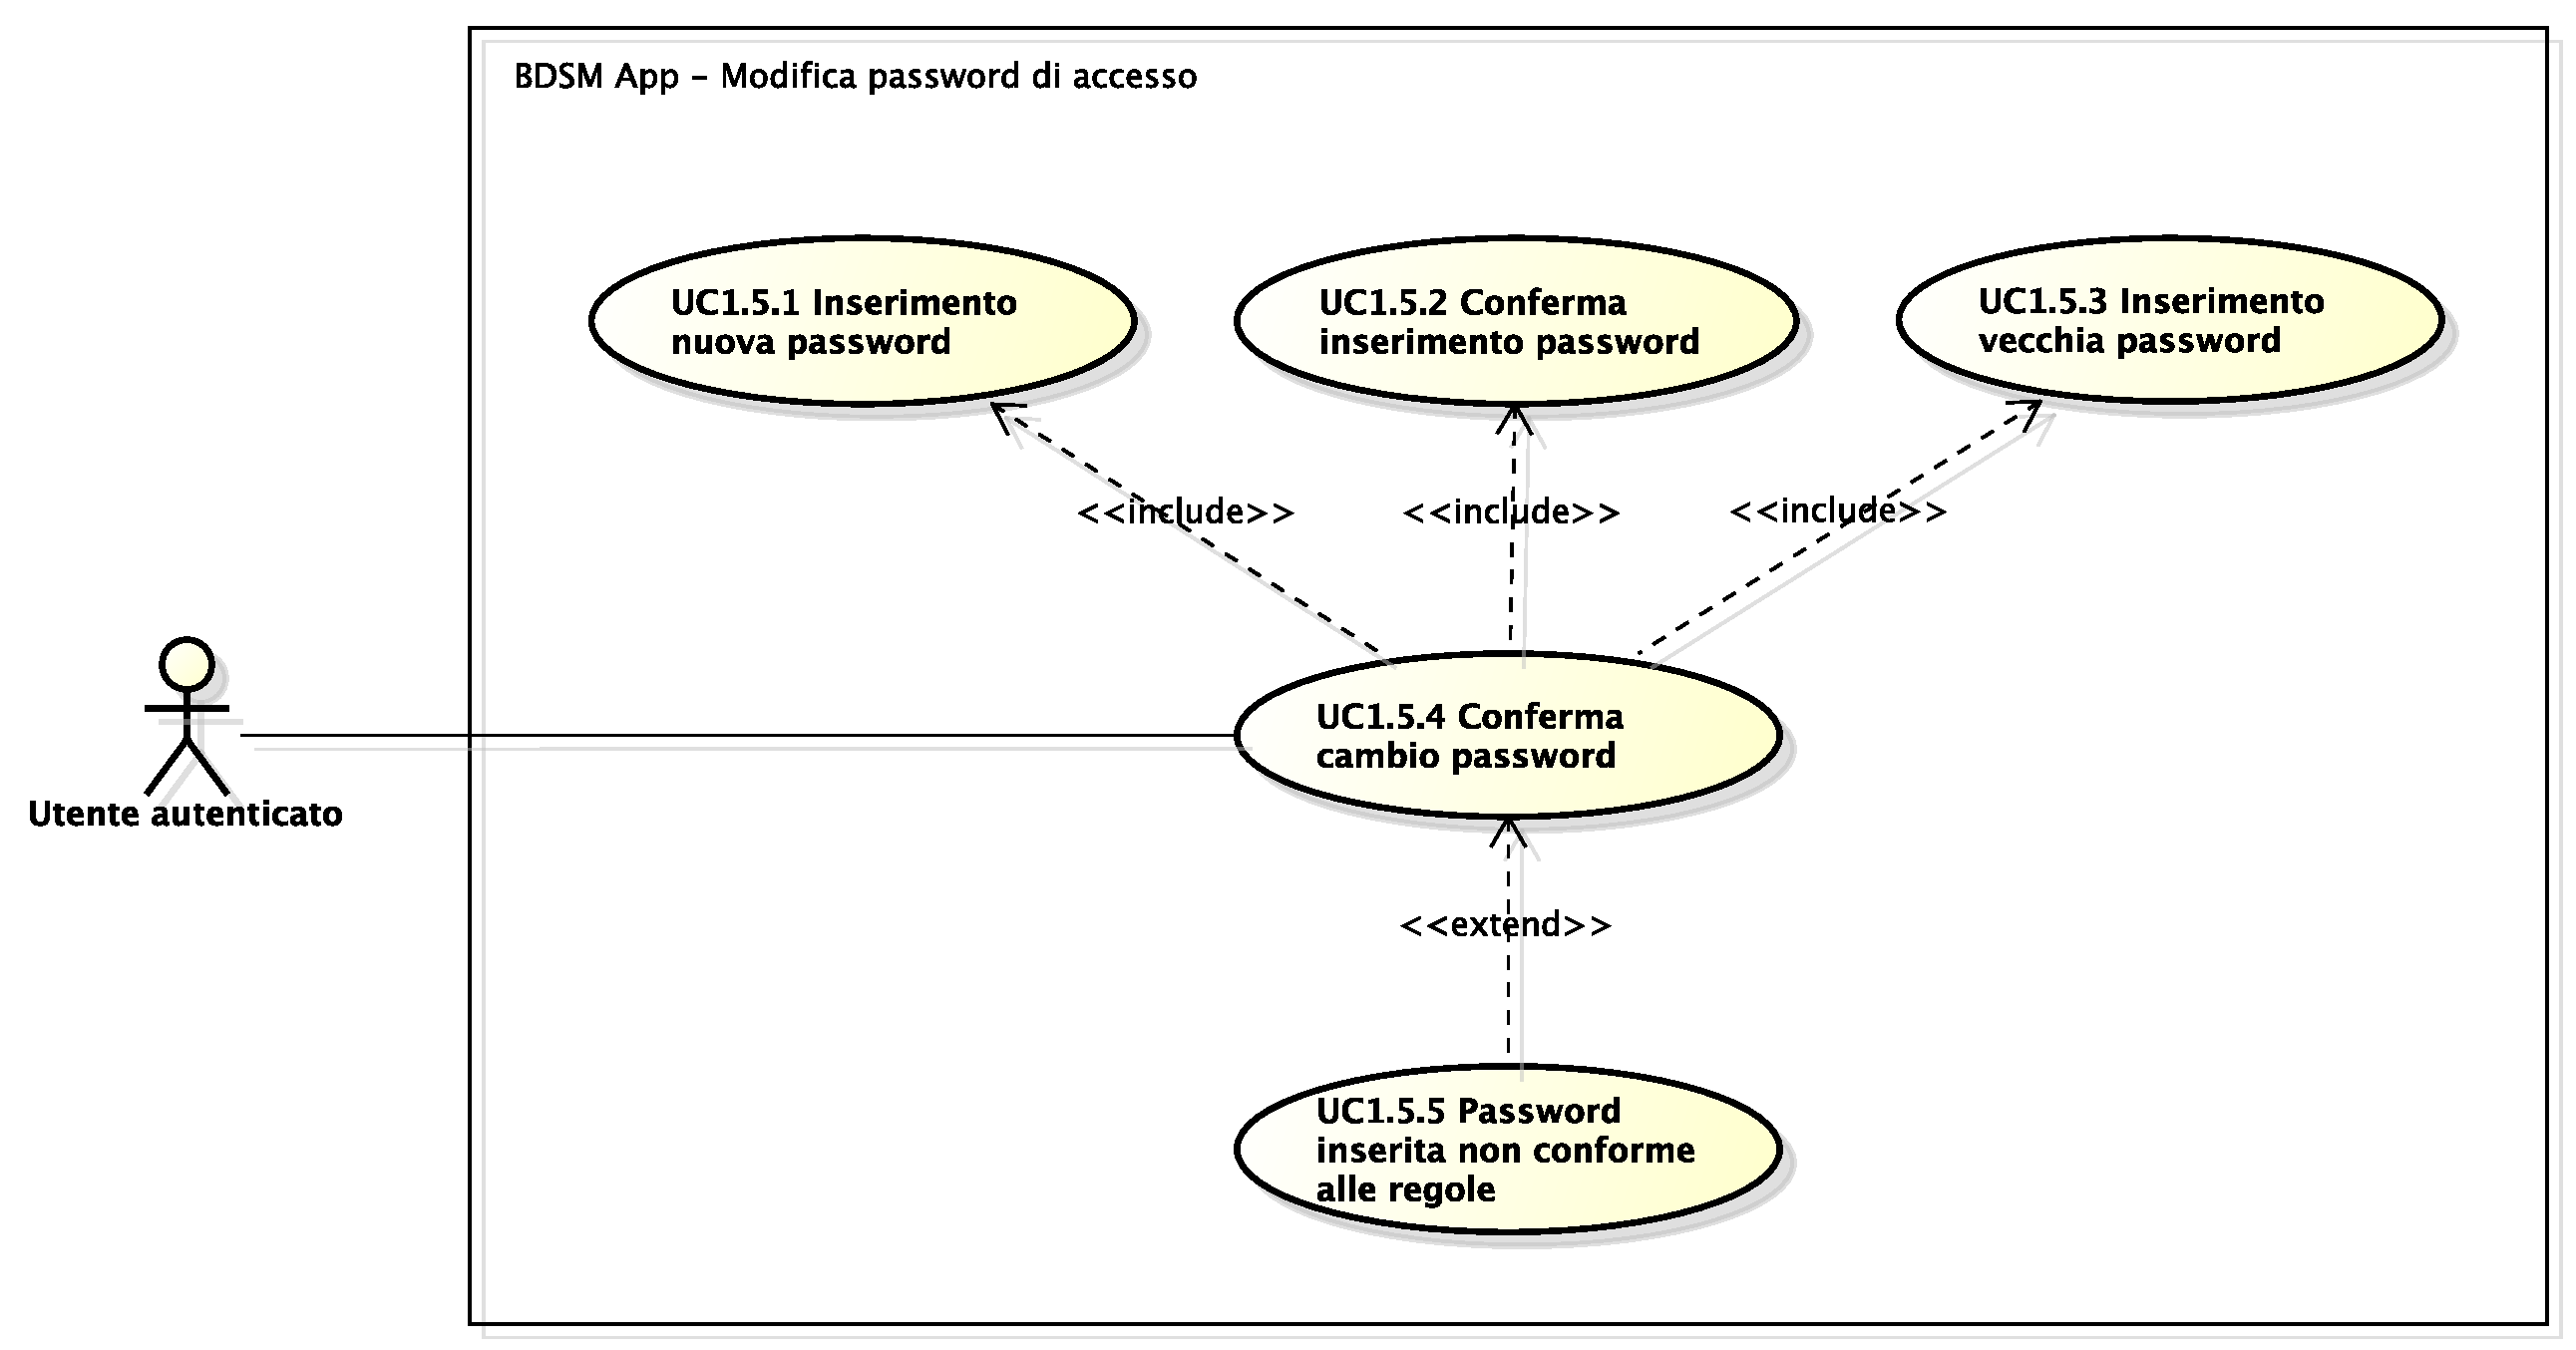
\includegraphics[scale=0.45]{./images/UC1_5.pdf}}
    \caption{UC1.5 - Modifica password di accesso}
\end{figure}

\begin{itemize}
   	\item \textbf{Attori:}
    \begin{itemize}
    	\item utente autenticato: utente autenticato che ha accesso al servizio;
    	\item utente amministratore: utente autenticato che ha accesso al servizio e dispone dei permessi per visualizzare tutte le aree;
	\end{itemize}
	  \item \textbf{Descrizione:} l'utente può cambiare la propria password selezionando il pulsante di cambio password nella sua home screen;
    \item \textbf{Precondizione:} l'utente dispone di una password di accesso valida, risulta autenticato al servizio e si trova nella sua home screen;
    \item \textbf{Postcondizione:} la nuova password per l'utente è attiva, la vecchia password non è più valida;
	\item \textbf{Flusso principale degli eventi:}
    \begin{enumerate}
        \item Inserimento nuova password (UC1.5.1);
        \item Conferma inserimento nuova password (UC1.5.2);
        \item Inserimento vecchia password (UC1.5.3);
        \item Conferma cambio password (UC1.5.4);
    \end{enumerate}
   	\item \textbf{Estensioni:} Password non corretta (UC1.5.5).

\end{itemize}

\subsubsection{UC1.5.1: Inserimento nuova password}

\begin{itemize}
   	\item \textbf{Attori:}
    \begin{itemize}
    	\item utente autenticato: utente autenticato che ha accesso al servizio;
    	\item utente amministratore: utente autenticato che ha accesso al servizio e dispone dei permessi per visualizzare tutte le aree;
	\end{itemize}
    \item \textbf{Descrizione:} l'utente può inserire la nuova password nel pannello apposito;
    \item \textbf{Precondizione:} l'utente ha selezionato il pulsante di cambio password nella sua home screen;
    \item \textbf{Postcondizione:} l'utente ha inserito la nuova password.
\end{itemize}

\subsubsection{UC1.5.2: Conferma inserimento password }

\begin{itemize}
   	\item \textbf{Attori:}
    \begin{itemize}
    	\item utente autenticato: utente autenticato che ha accesso al servizio;
    	\item utente amministratore: utente autenticato che ha accesso al servizio e dispone dei permessi per visualizzare tutte le aree;
	\end{itemize}
    \item \textbf{Descrizione:} l'utente deve inserire nuovamente la nuova password per verificare di non aver fatto errori di battitura;
    \item \textbf{Precondizione:} l'utente ha inserito la nuova password;
    \item \textbf{Postcondizione:} l'utente ha verificato la correttezza della nuova password.
\end{itemize}

\subsubsection{UC1.5.3: Inserimento vecchia password}

\begin{itemize}
    	\item \textbf{Attori:}
    \begin{itemize}
    	\item utente autenticato: utente autenticato che ha accesso al servizio;
    	\item utente amministratore: utente autenticato che ha accesso al servizio e dispone dei permessi per visualizzare tutte le aree;
	\end{itemize}
    \item \textbf{Descrizione:} l'utente deve inserire la vecchia password per completare il cambio password;
    \item \textbf{Precondizione:} l'utente ha inserito la nuova password due volte negli appositi campi;
    \item \textbf{Postcondizione:} l'utente ha inserito la vecchia password e può confermare la nuova.
\end{itemize}

\subsubsection{UC1.5.4: Conferma cambio password}

\begin{itemize}
   	\item \textbf{Attori:}
    \begin{itemize}
    	\item utente autenticato: utente autenticato che ha accesso al servizio;
    	\item utente amministratore: utente autenticato che ha accesso al servizio e dispone dei permessi per visualizzare tutte le aree;
	\end{itemize}
    \item \textbf{Descrizione:} l'utente deve confermare di voler sostituire la vecchia password di accesso con quella nuova selezionando il pulsante di conferma;
    \item \textbf{Precondizione:} l'utente ha inserito due volte la nuova password ed una la vecchia negli appositi campi;
    \item \textbf{Postcondizione:} l'utente ha confermato l'operazione e la nuova password è ora attiva.
\end{itemize}

\subsubsection{UC1.5.5: Password non corretta}

\begin{itemize}
   	\item \textbf{Attori:}
    \begin{itemize}
    	\item utente autenticato: utente autenticato che ha accesso al servizio;
    	\item utente amministratore: utente autenticato che ha accesso al servizio e dispone dei permessi per visualizzare tutte le aree;
	\end{itemize}
    \item \textbf{Descrizione:} l'utente può aver inserito una password che non soddisfa i vincoli di sistema specificati nel pannello di cambio password;
    \item \textbf{Precondizione:} l'utente ha selezionato il pulsante di conferma del cambio password;
    \item \textbf{Postcondizione:} l'utente ha visualizzato un messaggio di errore con i dettagli dei vincoli non soddisfatti.
\end{itemize}

\pagebreak


\subsection{UC1.6: Logout utente}

\begin{figure}[htbp]
    \centering
    \centerline{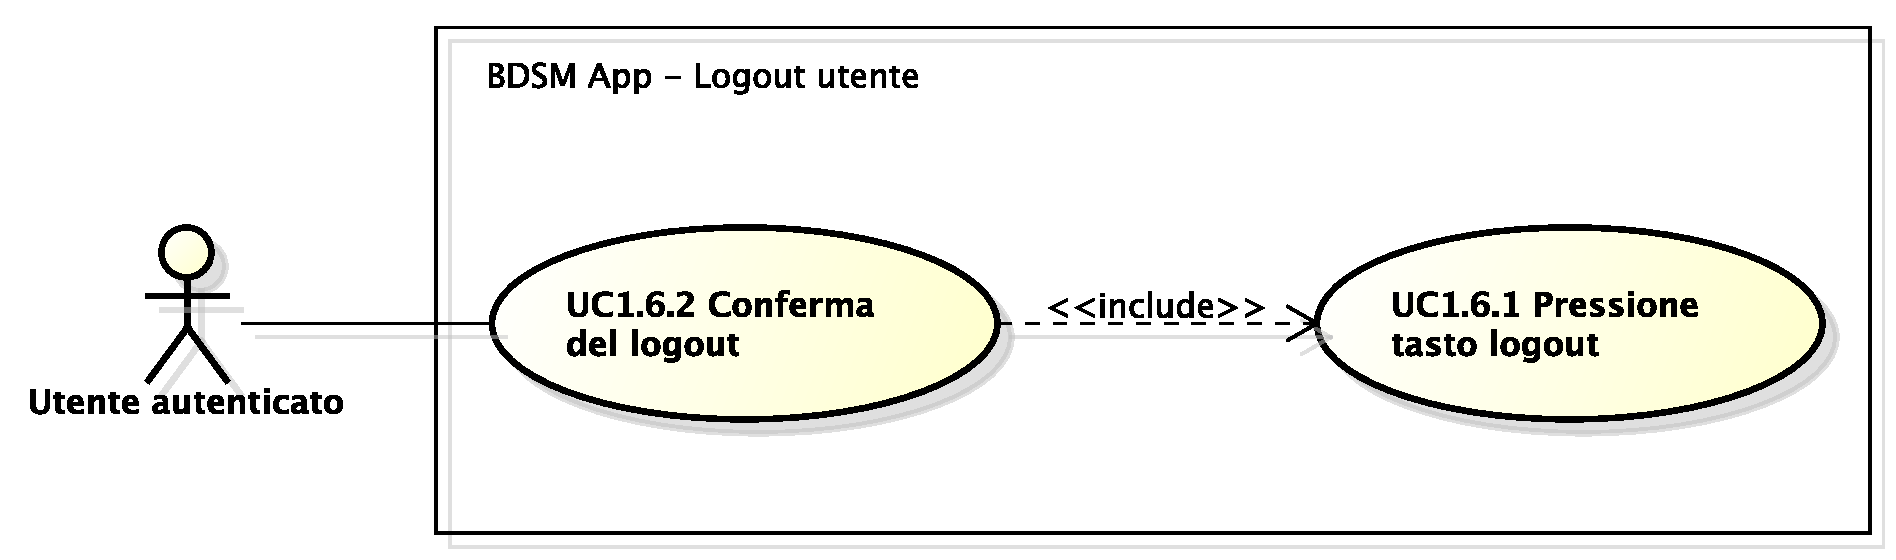
\includegraphics[scale=0.45]{./images/UC1_6.pdf}}
    \caption{UC1.6 - Logout utente}
\end{figure}

\begin{itemize}
   	\item \textbf{Attori:}
    \begin{itemize}
    	\item utente autenticato: utente autenticato che ha accesso al servizio;
    	\item utente amministratore: utente autenticato che ha accesso al servizio e dispone dei permessi per visualizzare tutte le aree;
	\end{itemize}
	\item \textbf{Descrizione:} l'utente può terminare la sessione di lavoro. Questa operazione può essere eseguita premendo il pulsante di logout nella home screen;
    \item \textbf{Precondizione:} l'utente risulta autenticato al servizio;
    \item \textbf{Postcondizione:} la sessione di lavoro è terminata. Viene mostrata la schermata di login;
    \item \textbf{Flusso principale degli eventi:}
    \begin{enumerate}
        \item Pressione tasto logout (UC1.6.1);
        \item Conferma del logout (UC1.6.2).
    \end{enumerate}
\end{itemize}

\subsubsection{UC1.6.1: Pressione tasto logout}

\begin{itemize}
   	\item \textbf{Attori:}
    \begin{itemize}
    	\item utente autenticato: utente autenticato che ha accesso al servizio;
    	\item utente amministratore: utente autenticato che ha accesso al servizio e dispone dei permessi per visualizzare tutte le aree;
	\end{itemize}
    \item \textbf{Descrizione:} l'utente può effettuare il logout selezionando l'apposito pulsante nella sua home screen;
    \item \textbf{Precondizione:} l'utente ha effettuato l'accesso al servizio e si trova nella home screen;
    \item \textbf{Postcondizione:} l'utente visualizza il pannello di conferma logout.
\end{itemize}

\subsubsection{UC1.6.2: Conferma del logout}

\begin{itemize}
   	\item \textbf{Attori:}
    \begin{itemize}
    	\item utente autenticato: utente autenticato che ha accesso al servizio;
    	\item utente amministratore: utente autenticato che ha accesso al servizio e dispone dei permessi per visualizzare tutte le aree;
	\end{itemize}
    \item \textbf{Descrizione:} prima di terminare la sessione di lavoro l'utente deve confermare la volontà di farlo selezionando il pulsante di conferma sul pannello di logout;
    \item \textbf{Precondizione:} l'utente ha selezionato il pulsante di logout nella home screen;
    \item \textbf{Postcondizione:} l'utente ha confermato il logout e la sessione è terminata. Viene visualizzata la schermata di login.
\end{itemize}

\pagebreak


\subsection{UC1.7: Amministrazione degli utenti}

\begin{figure}[!htbp]
    \centering
    \centerline{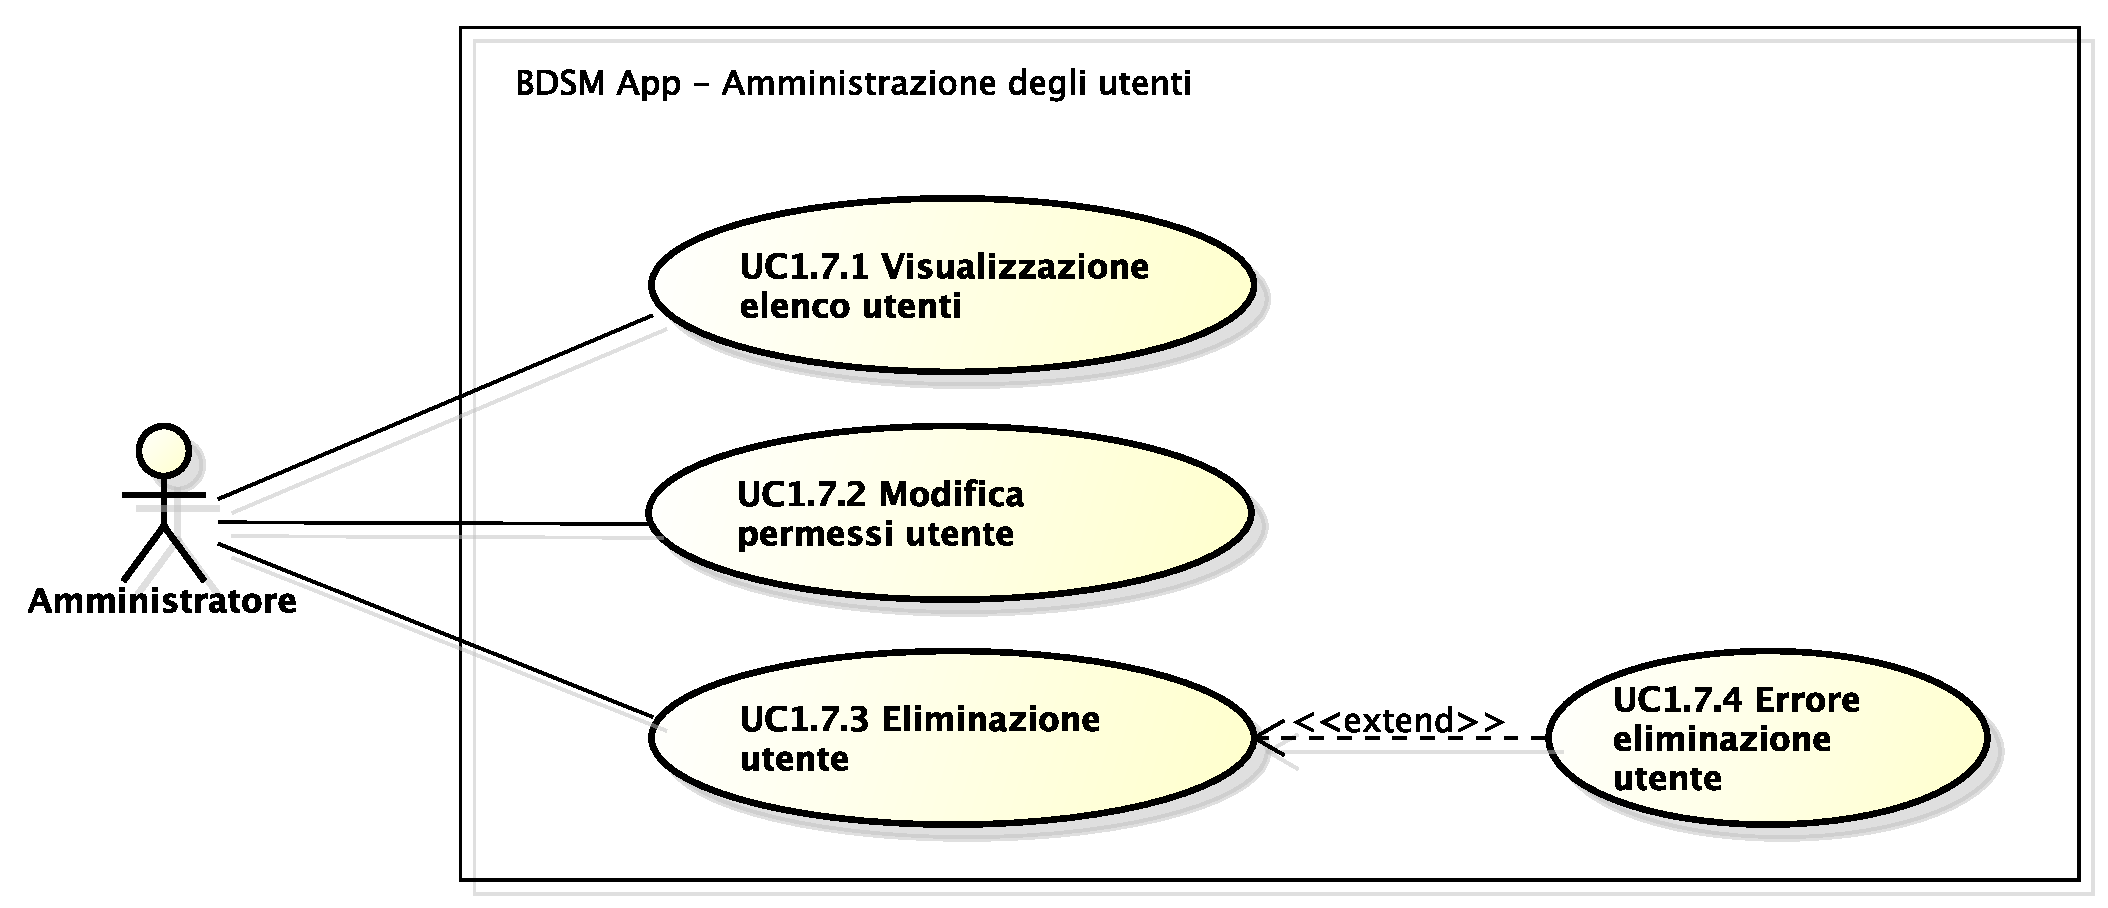
\includegraphics[scale=0.45]{./images/UC1_7.pdf}}
    \caption{UC1.7 - Amministrazioni degli utenti}
\end{figure}

\begin{itemize}
    \item \textbf{Attori:} utente amministratore: utente autenticato che ha accesso al servizio e dispone dei permessi per visualizzare tutte le aree;
    \item \textbf{Descrizione:} l'amministratore può gestire i permessi di accesso di un altro utente. Può anche eliminare definitivamente un utente e tutte le sue View\gloss{};
    \item \textbf{Precondizione:} l'amministratore ha effettuato l'accesso al sistema;
    \item \textbf{Postcondizione:} il sistema ha eseguito le operazioni richieste;
    \item \textbf{Flusso principale degli eventi:}
    \begin{enumerate}
        \item Visualizzazione elenco utenti (UC1.7.1);
        \item Modifica permessi utente (UC1.7.2);
        \item Eliminazione utente (UC1.7.3);
    \end{enumerate}
    \item \textbf{Estensioni:} Errore eliminazione utente (UC1.7.4).
\end{itemize}

\subsubsection{UC1.7.1: Visualizzazione elenco utenti}

\begin{itemize}
    \item \textbf{Attori:} utente amministratore: utente autenticato che ha accesso al servizio e dispone dei permessi per visualizzare tutte le aree;
    \item \textbf{Descrizione:} l'amministratore può visualizzare l'elenco di tutti gli utenti salvati nel sistema selezionando l'apposito pulsante nella sua home screen;
    \item \textbf{Precondizione:} l'amministratore ha effettuato l'accesso al sistema e si trova nella sua home screen;
    \item \textbf{Postcondizione:} l'amministratore ha visualizzato l'elenco degli utenti.
\end{itemize}

\subsubsection{UC1.7.2: Modifica permessi utente}

\begin{itemize}
    \item \textbf{Attori:} utente amministratore: utente autenticato che ha accesso al servizio e dispone dei permessi per visualizzare tutte le aree;
    \item \textbf{Descrizione:} l'amministratore può cambiare i permessi di accesso al sistema ad un utente diverso da se stesso;
    \item \textbf{Precondizione:} l'amministratore ha eseguito l'accesso;
    \item \textbf{Postcondizione:} l'amministratore ha modificato i permessi ad un utente;
    \item \textbf{Flusso principale degli eventi:}
    \begin{enumerate}
        \item Apertura elenco utenti (UC1.7.2.1);
        \item Apertura pannello modifica permessi(UC1.7.2.2);
        \item Selezione nuovi permessi (UC1.7.2.3);
        \item Conferma modifiche (UC1.7.2.4).
    \end{enumerate}
\end{itemize}

\subsubsection{UC1.7.2.1: Apertura elenco utenti}

\begin{itemize}
    \item \textbf{Attori:} utente amministratore: utente autenticato che ha accesso al servizio e dispone dei permessi per visualizzare tutte le aree;
    \item \textbf{Descrizione:} l'amministratore può visualizzare l'elenco degli utenti salvati nel sistema selezionando l'apposito pulsante nella sua home screen;
    \item \textbf{Precondizione:} l'amministratore ha effettuato l'accesso al sistema e si trova nella sua home screen;
    \item \textbf{Postcondizione:} l'amministratore ha visualizzato l'elenco degli utenti.
\end{itemize}

\subsubsection{UC1.7.2.2: Apertura pannello modifica permessi}

\begin{itemize}
    \item \textbf{Attori:} utente amministratore: utente autenticato che ha accesso al servizio e dispone dei permessi per visualizzare tutte le aree;
    \item \textbf{Descrizione:} l'amministratore può cambiare i permessi di accesso ad un utente premendo l'apposito pulsante nell'elenco utenti;
    \item \textbf{Precondizione:} l'amministratore ha visualizzato l'elenco utenti;
    \item \textbf{Postcondizione:} l'amministratore ha selezionato il pulsante di modifica permessi di un utente.
\end{itemize}

\subsubsection{UC1.7.2.3: Selezione nuovi permessi}

\begin{itemize}
    \item \textbf{Attori:} utente amministratore: utente autenticato che ha accesso al servizio e dispone dei permessi per visualizzare tutte le aree;
    \item \textbf{Descrizione:} l'amministratore può cambiare i permessi per l'utente selezionato;
    \item \textbf{Precondizione:} l'amministratore ha premuto il pulsante di modifica permessi utente;
    \item \textbf{Postcondizione:} l'amministratore ha selezionato i nuovi permessi per l'utente.
\end{itemize}

\subsubsection{UC1.7.2.4: Conferma modifiche}

\begin{itemize}
    \item \textbf{Attori:} utente amministratore: utente autenticato che ha accesso al servizio e dispone dei permessi per visualizzare tutte le aree;
    \item \textbf{Descrizione:} l'amministratore ha confermato le modifiche ai permessi dell'utente;
    \item \textbf{Precondizione:} l'amministratore ha selezionato nuovi permessi per l'utente;
    \item \textbf{Postcondizione:} l'amministratore ha confermato le modifiche e sono ora attive nel sistema.
\end{itemize}

\subsubsection{UC1.7.3: Eliminazione utente}

\begin{itemize}
    \item \textbf{Attori:} utente amministratore: utente autenticato che ha accesso al servizio e dispone dei permessi per visualizzare tutte le aree;
    \item \textbf{Descrizione:} l'amministratore può eliminare un utente e tutte le sue View\gloss{} dal sistema;
    \item \textbf{Precondizione:} l'amministratore ha eseguito l'accesso;
    \item \textbf{Postcondizione:} l'amministratore ha cancellato un utente e le sue View\gloss{};
    \item \textbf{Flusso principale degli eventi:}
    \begin{enumerate}
        \item Apertura elenco utenti (UC1.7.3.1);
        \item Selezione pulsante elimina (UC1.7.3.2);
        \item Conferma eliminazione (UC1.7.3.3).
    \end{enumerate}
\end{itemize}

\subsubsection{UC1.7.3.1: Apertura elenco utenti}

\begin{itemize}
    \item \textbf{Attori:} utente amministratore: utente autenticato che ha accesso al servizio e dispone dei permessi per visualizzare tutte le aree;
    \item \textbf{Descrizione:} l'amministratore può visualizzare l'elenco di tutti gli utenti salvati nel sistema selezionando l'apposito pulsante nella sua home screen;
    \item \textbf{Precondizione:} l'amministratore ha effettuato l'accesso al sistema e si trova nella sua home screen;
    \item \textbf{Postcondizione:} l'amministratore ha visualizzato l'elenco degli utenti.
\end{itemize}

\subsubsection{UC1.7.3.2: Selezione pulsante elimina}

\begin{itemize}
    \item \textbf{Attori:} utente amministratore: utente autenticato che ha accesso al servizio e dispone dei permessi per visualizzare tutte le aree;
    \item \textbf{Descrizione:} l'amministratore può avviare la procedura di eliminazione selezionando il pulsante elimina utente;
    \item \textbf{Precondizione:} l'amministratore ha visualizzato l'elenco degli utenti;
    \item \textbf{Postcondizione:} l'amministratore ha visualizzato il pannello di conferma eliminazione.
\end{itemize}

\subsubsection{UC1.7.3.3: Conferma eliminazione}

\begin{itemize}
    \item \textbf{Attori:} utente amministratore: utente autenticato che ha accesso al servizio e dispone dei permessi per visualizzare tutte le aree;
    \item \textbf{Descrizione:} l'amministratore deve confermare l'eliminazione dell'utente;
    \item \textbf{Precondizione:} l'amministratore ha aperto il pannello di conferma eliminazione utente;
    \item \textbf{Postcondizione:} l'utente selezionato è stato cancellato dal sistema insieme a tutte le sue View\gloss{}.
\end{itemize}

\subsubsection{UC1.7.4: Errore eliminazione utente}


\begin{itemize}
    \item \textbf{Attori:} utente amministratore: utente autenticato che ha accesso al servizio e dispone dei permessi per visualizzare tutte le aree;
    \item \textbf{Descrizione:} l'amministratore può visualizzare un messaggio di errore se l'utente che vuole eliminare è attualmente autenticato nel sistema e sta eseguendo delle operazioni;
    \item \textbf{Precondizione:} l'amministratore ha confermato l'eliminazione di un utente;
    \item \textbf{Postcondizione:} l'amministratore ha visualizzato il messaggio di errore. Nessun utente o dato è stato eliminato dal sistema.
\end{itemize}

\pagebreak


\subsection{UC1.8: Registrazione nuovo utente}

\begin{figure}[!htbp]
    \centering
    \centerline{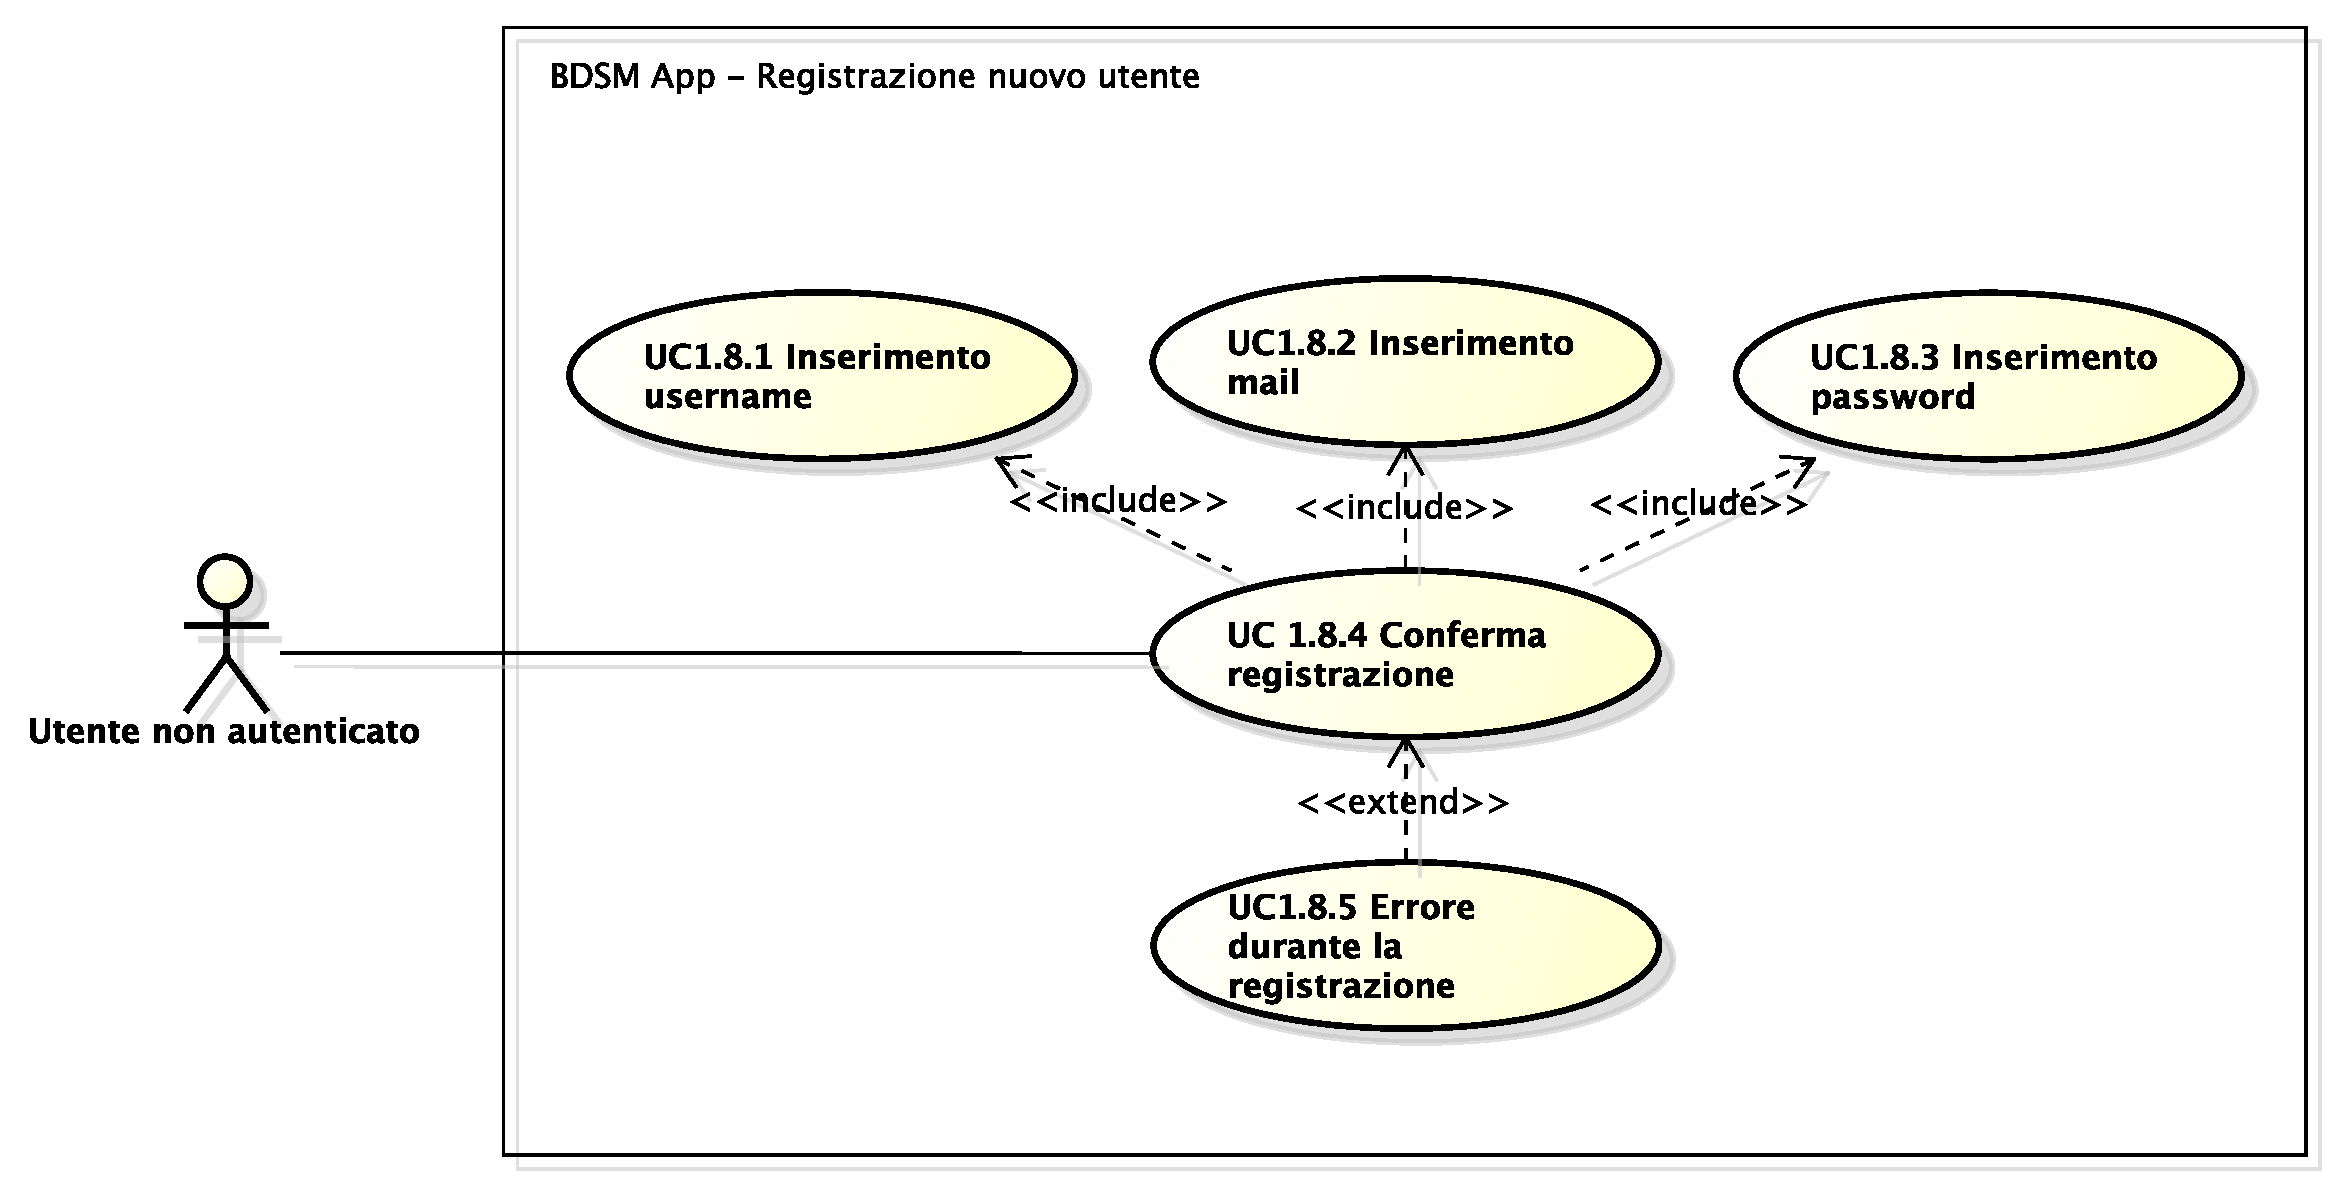
\includegraphics[scale=0.45]{./images/UC1_8.pdf}}
    \caption{UC1.8 - Registrazione nuovo utente}
\end{figure}

\begin{itemize}
   	\item \textbf{Attori:} utente sconosciuto: utente non autenticato che accede al servizio;
    \item \textbf{Descrizione:} un utente deve poter creare un account per poter eseguire il login
    all'interno del sistema e usufruire delle funzionalità offerte;
    \item \textbf{Precondizione:} l'utente accede al sito web tramite un browser supportato
    dal sistema;
    \item \textbf{Postcondizione:} il sistema ha memorizzato i dati relativi al nuovo account e
    ripresenta all'utente la schermata iniziale;
    \item \textbf{Flusso principale degli eventi:}
    \begin{enumerate}
        \item Inserimento username (UC1.8.1);
        \item Inserimento email (UC1.8.2);
        \item Inserimento password (UC1.8.3);
        \item Conferma registrazione (UC1.8.4);
    \end{enumerate}
    \item \textbf{Estensioni:} Errore durante la registrazione (UC1.8.5).
\end{itemize}


\subsubsection{UC1.8.1: Inserimento username}

\begin{itemize}
   	\item \textbf{Attori:} utente sconosciuto: utente non autenticato che accede al servizio;
    \item \textbf{Descrizione:} l'utente deve inserire il proprio nome utente per essere riconoscibile univocamente all'interno del sistema e per poter gestire le proprie View\gloss{};
    \item \textbf{Precondizione:} il sistema fornisce una schermata in cui è possibile inserire l'username per il nuovo account;
    \item \textbf{Postcondizione:} l'utente ha inserito il proprio username.
\end{itemize}

\subsubsection{UC1.8.2: Inserimento mail}

\begin{itemize}
   	\item \textbf{Attori:} utente sconosciuto: utente non autenticato che accede al servizio;
    \item \textbf{Descrizione:} l'utente deve inserire la mail che vuole associare alle username appena inserito;
    \item \textbf{Precondizione:} il sistema fornisce una schermata in cui è possibile inserire la mail per il nuovo account;
    \item \textbf{Postcondizione:} l'utente ha inserito il proprio indirizzo mail.
\end{itemize}

\subsubsection{UC1.8.3: Inserimento password}

\begin{itemize}
   	\item \textbf{Attori:} utente sconosciuto: utente non autenticato che accede al servizio;
    \item \textbf{Descrizione:} l'utente deve inserire la password che vuole associare ai dati precedetemente inseriti;
    \item \textbf{Precondizione:} il sistema fornisce una schermata in cui è possibile inserire la password per il nuovo account;
    \item \textbf{Postcondizione:} l'utente ha inserito la password.
\end{itemize}

\subsubsection{UC1.8.4: Conferma registrazione}

\begin{itemize}
   	\item \textbf{Attori:} utente sconosciuto: utente non autenticato che accede al servizio;
    \item \textbf{Descrizione:} l'utente deve poter confermare i dati inseriti durante la registrazione;
    \item \textbf{Precondizione:} il sistema fornisce una schermata in cui è possibile confermare i dati inseriti in precedenza per la creazione di un nuovo account;
    \item \textbf{Postcondizione:} l'utente ha confermato di voler creare un nuovo account all'interno
    del sistema.
\end{itemize}

\subsubsection{UC1.8.5: Errore durante la registrazione}

\begin{itemize}
   	\item \textbf{Attori:} utente sconosciuto: utente non autenticato che accede al servizio;
    \item \textbf{Descrizione:} se vengono inseriti dei dati non conformi ai vincoli di sistema indicati durante la registrazione viene visualizzata una schermata di errore;
    \item \textbf{Precondizione:} i dati inseriti non rispettano uno o più vincoli di sistema;
    \item \textbf{Postcondizione:} l'utente ha visualizzato l'errore relativo ai dati inseriti.
\end{itemize}

\pagebreak
